\documentclass[11pt,oneside]{article}

\usepackage[a4paper,margin=27mm,headheight=15pt]{geometry}
\usepackage[T1]{fontenc}
\usepackage[utf8]{inputenc}
\IfFileExists{libertinus.sty}{\usepackage{libertinus}}{\usepackage{lmodern}}
\usepackage{microtype}
\usepackage{amsmath,amssymb,amsthm,mathtools,mathrsfs}
% Canonical mathematical notation for active FabiusFunction LaTeX documents.
%
% This file is intentionally a plain TeX input rather than a LaTeX package.
% Every standalone document loads it by an explicit path relative to that
% document's directory; included fragments inherit the definitions from their
% root document.  Keep this file independent of document layout and metadata.
%
% Contract:
%   * one command has one mathematical meaning throughout the active corpus;
%   * names encode semantic roles rather than a document-local choice of letter;
%   * visually similar but differently normalized objects have different print;
%   * every command below is defined normatively in the notation catalogue.
%
% The active corpus excludes docs/archive/.  Historical sources may retain
% their original notation only inside an explicitly labelled quotation.

\makeatletter
\@ifundefined{mathbb}{%
  \PackageError{fabius-notation}{The amssymb package must be loaded first}%
    {Load amsmath and amssymb before inputting fabius-notation.tex.}%
}{}
\@ifundefined{operatorname}{%
  \PackageError{fabius-notation}{The amsmath package must be loaded first}%
    {Load amsmath before inputting fabius-notation.tex.}%
}{}
\makeatother

% Version stamp used by the catalogue and by static audits.
\newcommand{\FabiusNotationVersion}{2026-08-31}

% Number systems.  NaturalNumbers is explicitly the nonnegative convention.
\newcommand{\NaturalNumbers}{\mathbb{N}_{0}}
\newcommand{\PositiveIntegers}{\mathbb{N}_{>0}}
\newcommand{\IntegerNumbers}{\mathbb{Z}}
\newcommand{\RationalNumbers}{\mathbb{Q}}
\newcommand{\RealNumbers}{\mathbb{R}}
\newcommand{\ComplexNumbers}{\mathbb{C}}
\newcommand{\ExtendedRealNumbers}{\overline{\mathbb{R}}}

% The three principal Fabius--Rvachev functions.  Subscripts are deliberate:
% a bare F and a calligraphic F have several unrelated uses in the corpus.
\newcommand{\FabiusBounded}{F_{\mathrm{bd}}}
\newcommand{\FabiusGlobal}{F_{\mathrm{gl}}}
\newcommand{\FabiusQuantile}{Q_{F}}
\newcommand{\FabiusClampedQuantile}{Q_{F,\mathrm{cl}}}
\newcommand{\RvachevUp}{\operatorname{up}}

% Constants, elementary operators, and delimiters.
\newcommand{\EulerE}{\mathrm{e}}
\newcommand{\ImaginaryUnit}{\mathrm{i}}
\newcommand{\Differential}{\mathop{}\!\mathrm{d}}
\newcommand{\AbsoluteValue}[1]{\left\lvert #1\right\rvert}
\newcommand{\Norm}[1]{\left\lVert #1\right\rVert}
\newcommand{\Floor}[1]{\left\lfloor #1\right\rfloor}
\newcommand{\Ceiling}[1]{\left\lceil #1\right\rceil}
\newcommand{\FractionalPart}[1]{\left\{#1\right\}}
\newcommand{\PositivePart}[1]{\left(#1\right)_{+}}
\newcommand{\IndicatorOf}[1]{\mathbf{1}_{#1}}
\newcommand{\SetOf}[1]{\left\{#1\right\}}
\newcommand{\InnerProduct}[1]{\left\langle #1\right\rangle}
\newcommand{\CardinalityOf}[1]{\left\lvert #1\right\rvert}
\newcommand{\DefinitionEquals}{\mathrel{\coloneqq}}
\newcommand{\Sign}{\operatorname{sgn}}
\newcommand{\IdentityOperator}{\operatorname{id}}
\newcommand{\SpanOperator}{\operatorname{span}}
\newcommand{\TraceOperator}{\operatorname{tr}}
\newcommand{\RankOperator}{\operatorname{rank}}
\newcommand{\DiagonalOperator}{\operatorname{diag}}
\newcommand{\ResidueOperator}{\operatorname*{Res}}
\newcommand{\LeastCommonMultiple}{\operatorname{lcm}}
\newcommand{\OrderOperator}{\operatorname{ord}}
\newcommand{\PrincipalLogarithm}{\operatorname{Log}}
\newcommand{\FallingFactorial}[2]{\left(#1\right)^{\underline{#2}}}
\newcommand{\RisingFactorial}[2]{\left(#1\right)^{\overline{#2}}}

% Support, topology, convolution, and metric notation.
\newcommand{\SupportOperator}{\operatorname{supp}}
\newcommand{\SupportOf}[1]{\SupportOperator\!\left(#1\right)}
\newcommand{\TopologicalSupportOf}[1]{\operatorname{tsupp}\!\left(#1\right)}
\newcommand{\Convolution}{\mathbin{*}}
\newcommand{\MetricDistance}{\operatorname{dist}}
\newcommand{\TotalVariationDistance}{d_{\mathrm{TV}}}

% Probability.  Equality and convergence in law are not metric distance.
\newcommand{\Probability}{\mathbb{P}}
\newcommand{\Expectation}{\mathbb{E}}
\newcommand{\Variance}{\operatorname{Var}}
\newcommand{\Covariance}{\operatorname{Cov}}
\newcommand{\LawOperator}{\operatorname{Law}}
\newcommand{\LawOf}[1]{\LawOperator\!\left(#1\right)}
\newcommand{\EqualInLaw}{\mathrel{\overset{\mathrm{law}}{=}}}
\newcommand{\ConvergesInLaw}{\mathrel{\xrightarrow{\mathrm{law}}}}

% Fourier and integral transforms.  The printed labels expose normalization.
% FourierTwoPi uses exp(-2*pi*i*x*xi); FourierAngular uses exp(-i*x*omega).
\newcommand{\FourierTwoPi}[1]{\widehat{#1}_{\,2\pi}}
\newcommand{\FourierAngular}[1]{\widehat{#1}_{\,\mathrm{ang}}}
\newcommand{\LaplaceTransformSymbol}{\mathcal{L}}
\newcommand{\MellinTransformSymbol}{\mathcal{M}}
\newcommand{\LaplaceTransformOf}[1]{\LaplaceTransformSymbol\!\left[#1\right]}
\newcommand{\MellinTransformOf}[1]{\MellinTransformSymbol\!\left[#1\right]}
\newcommand{\MomentGeneratingFunction}[1]{M_{#1}}
\newcommand{\CharacteristicFunction}[1]{\varphi_{#1}}

% The two standard sinc functions must never share one symbol.
\newcommand{\SincRad}{\operatorname{sinc}_{\mathrm{rad}}}
\newcommand{\SincPi}{\operatorname{sinc}_{\pi}}

% Binary arithmetic and Thue--Morse notation.
\newcommand{\BinaryDigitSum}{\operatorname{wt}_{2}}
\newcommand{\ThueMorseSignSymbol}{\varepsilon}
\newcommand{\ThueMorseSign}[1]{\varepsilon_{#1}}
\newcommand{\PadicValuation}[1]{\nu_{#1}}
\newcommand{\TwoAdicValuation}{\nu_{2}}

% q-series notation.  Every base is an explicit argument.
\newcommand{\QPochhammer}[3]{\left(#1;#2\right)_{#3}}
\newcommand{\GaussianBinomial}[3]{%
  \genfrac{[}{]}{0pt}{}{#1}{#2}_{#3}%
}
\newcommand{\QInteger}[2]{\left[#1\right]_{#2}}

% Named special functions.
\newcommand{\Polylogarithm}{\operatorname{Li}}
\newcommand{\LambertW}{W}
\newcommand{\GammaFunction}{\Gamma}
\newcommand{\RiemannZeta}{\zeta}

% Asymptotics.  BigO and LittleO are operator tokens for existing formula
% grammar; prefer the At forms so that the limiting regime is printed.
\newcommand{\BigO}{\mathcal{O}}
\newcommand{\LittleO}{o}
\newcommand{\BigOAt}[2]{\mathcal{O}_{#2}\!\left(#1\right)}
\newcommand{\LittleOAt}[2]{o_{#2}\!\left(#1\right)}

\usepackage{bm}
\usepackage{booktabs,longtable,array,tabularx}
\usepackage{graphicx}
\usepackage{pgfplots}
\usepackage{xcolor}
\usepackage{enumitem}
\usepackage{fancyhdr}
\usepackage{titlesec}
\usepackage{listings}
\usepackage{xurl}
\usepackage{hyperref}
\usepackage[nameinlink,noabbrev]{cleveref}

\definecolor{linkblue}{RGB}{25,75,135}
\definecolor{shadegray}{RGB}{246,247,249}
\definecolor{rulegray}{RGB}{195,201,208}
\pgfplotsset{compat=1.18}
\hypersetup{
  colorlinks=true,
  linkcolor=linkblue,
  citecolor=linkblue,
  urlcolor=linkblue,
  pdftitle={Zero-Bias Towers and Spectral Peeling in the Fabius--Rvachev System},
  pdfsubject={New probability, spectral-arithmetic, q-series, and endpoint-asymptotic structures},
  pdfkeywords={Fabius function, Rvachev up-function, zero bias, Thue-Morse, q-Pochhammer, Laguerre-Polya, Lambert W, mod-Gamma}
}

\pagestyle{fancy}
\fancyhf{}
\fancyhead[L]{\small Zero-bias towers in the Fabius--Rvachev system}
\fancyhead[R]{\small\nouppercase{\leftmark}}
\fancyfoot[C]{\thepage}
\renewcommand{\headrulewidth}{0.4pt}

\titleformat{\section}{\Large\bfseries}{\thesection}{0.7em}{}
\titleformat{\subsection}{\large\bfseries}{\thesubsection}{0.7em}{}
\titleformat{\subsubsection}{\normalsize\bfseries}{\thesubsubsection}{0.7em}{}
\setcounter{secnumdepth}{3}
\setcounter{tocdepth}{2}
\setlist[itemize]{leftmargin=2em,itemsep=0.25em,topsep=0.4em}
\setlist[enumerate]{leftmargin=2.3em,itemsep=0.25em,topsep=0.4em}

% Long unbreakable inline mathematics occasionally leaves a line with no legal
% break point.  A small emergency stretch lets TeX loosen such a line rather
% than let it protrude into the margin; it applies only to lines that would
% otherwise be overfull.
\setlength{\emergencystretch}{2em}

\newtheorem{theorem}{Theorem}[section]
\newtheorem{proposition}[theorem]{Proposition}
\newtheorem{lemma}[theorem]{Lemma}
\newtheorem{corollary}[theorem]{Corollary}
\newtheorem{conjecture}[theorem]{Conjecture}
\theoremstyle{definition}
\newtheorem{definition}[theorem]{Definition}
\newtheorem{algorithm}[theorem]{Algorithm}
\newtheorem{example}[theorem]{Example}
\theoremstyle{remark}
\newtheorem{remark}[theorem]{Remark}
\newtheorem{warning}[theorem]{Warning}

% Report-local notation and environments.
\graphicspath{{figures/}}
\allowdisplaybreaks
\newcommand{\Wass}{W_1}
\newcommand{\LP}{\mathcal{LP}}
\newcommand{\Dop}{\mathscr D}
\newcommand{\Tower}[1]{Y^{\langle #1\rangle}}
\newcommand{\repo}{\texttt{ProveIt}}

\newenvironment{proofidea}{\par\smallskip\noindent\textit{Proof architecture.}\ }{\hfill$\square$\par\smallskip}
\newenvironment{statusbox}{%
  \par\smallskip\noindent\begin{center}\begin{minipage}{0.94\textwidth}%
  \hrule\vspace{0.6em}\small
}{%
  \vspace{0.6em}\hrule\end{minipage}\end{center}\smallskip
}

\lstdefinestyle{python}{
  language=Python,
  basicstyle=\ttfamily\small,
  backgroundcolor=\color{shadegray},
  frame=single,
  rulecolor=\color{rulegray},
  columns=fullflexible,
  keepspaces=true,
  showstringspaces=false,
  breaklines=true,
  xleftmargin=0.7em,
  xrightmargin=0.7em,
  aboveskip=0.8em,
  belowskip=0.8em
}

\title{\bfseries Zero-Bias Towers and Spectral Peeling\\[0.3em]
\Large in the Fabius--Rvachev System\\[0.55em]
\large Random-index $q$-calculus, normalized Laguerre--P\'olya derivatives,\\
Thue--Morse release values, and logarithmic Gaussianization}
\author{Frontier research report for Vladimir Reshetnikov's \texttt{ProveIt} corpus}
\date{Repository-relative novelty audit through commit\\
\texttt{40fdea4cc0a728189f357389e3f114a2cb00e561} (30 August 2026)}

\begin{document}
\maketitle

\begin{abstract}
Let
\[
  Y=\sum_{j\ge1}2^{-j}U_j,
  \qquad U_j\stackrel{\mathrm{iid}}\sim\operatorname{Unif}[-1,1],
\]
so that $Y$ has Rvachev density $\RvachevUp$, while $X=(Y+1)/2$ has the Fabius
distribution function.  This report studies the iterated zero-bias tower
$Y=Y^{\langle0\rangle},Y^{\langle1\rangle},Y^{\langle2\rangle},\ldots$,
defined by
\(
 \Expectation[Wf(W)]=\Variance(W)\Expectation[f'(W^z)]
\)
at each symmetric level.  The direction was selected only after a recursive
search and manifest-level audit of the full \texttt{Analysis/FabiusFunction/docs}
LaTeX corpus.  General zero-biasing is classical; the claims of novelty below
are deliberately repository-relative and concern its exact synthesis with the
Fabius--Rvachev structures.

The tower admits a closed density kernel, an exact moment formula, and the
factorization
\[
 Y^{\langle m\rangle}\ \stackrel d=\ R_m B_m,
\]
where $R_m$ is the $2m$-power-biased radius $|Y|$ and $B_m$ is the first
coordinate of a uniform point of the sphere $S^{2m}$.  If
\[
 H(z)=\widehat{\RvachevUp}(\ImaginaryUnit\sqrt z/\pi),
\]
then every normalized derivative $H^{(m)}(z)/H^{(m)}(0)$ is exactly the
square-moment generating transform of $Y^{\langle m\rangle}$.  Consequently,
the Laguerre--P\'olya and P\'olya-frequency results already established for $H$
propagate to a probabilistically meaningful hierarchy.

For the geometric family
\(
Y_q=(1-q)\sum_{j\ge0}q^jU_j
\), one zero-bias step replaces a random digit whose index is geometric with
ratio $q^2$.  At level $m$, the numbers of replacements at the individual
digits have an exact occupancy law.  The probability that all $m$ hits occur
at distinct digits is
\[
 \frac{(2m-1)!!\,m!}{\mu_{2m}(q)3^m}
 \frac{(1-q)^{2m}q^{m(m-1)}}{(q^2;q^2)_m},
\]
which exposes a new $q$-Pochhammer layer inside the zero-bias dynamics.

The derivative hierarchy also peels the arithmetic Fourier divisor.  At the
lattice frequency $2\pi N$, the original characteristic function has order
$\nu_2(N)+1$.  Every tower step removes exactly one inherited order, and at the
first nonzero level the released value has a closed product formula whose sign
is
\(
(-1)^{\nu_2(N)+2+s_2((u-1)/2)}
\), where $u$ is the odd part of $N$.  Thus the Thue--Morse sequence controls
not merely signs between zeros, but the first value exposed after a multiple
zero is differentiated away.

Finally, the tower Gaussianizes every compact symmetric law whose support
reaches its endpoints:
\(
\sqrt{2m}\,Y^{\langle m\rangle}\Rightarrow N(0,1)
\).
For the Rvachev law the convergence is logarithmically slow.  The exact
negative-Laplace decomposition of the Fabius law yields a phase-dependent
mod-Gamma law for $2m(1-R_m)$ and the sharp transport scale
\[
 W_1\!\left(\sqrt{2m}\,Y^{\langle m\rangle},N(0,1)\right)
 \sim \sqrt{\frac2\pi}\,
       \frac{\log(2m)}{2m\log2}.
\]
The report ends with conjectures on spectral non-reappearance, Bessel--Airy
zero transitions, occupancy limit shapes, phase-resolved all-order expansions,
and a concrete Lean formalization program.  A fully commented Python program
reproduces the tables, exact rational checks, Monte Carlo occupancy sampler,
and figures.
\end{abstract}

\tableofcontents
\newpage

\section{Scope, corpus audit, and claim discipline}
\label{sec:scope}

The repository subtree examined for this report is
\path{Analysis/FabiusFunction/docs}, recursively.  The indexed tree contains
more than ninety LaTeX sources and generated LaTeX fragments, in addition to
Python, Lean, CSV, PDF, and archival assets.  It is not a single article but a
research library: a primary exposition, a mathematical glossary, a Lean
walkthrough, a q-special-function survey, endpoint and inverse asymptotics,
Fourier-decay reports, dyadic-comb studies, integration and transform volumes,
Legendre and Lagrange representation projects, spectral-arithmetic reports,
Stein--Koopman work, and several consolidated frontier compilations.

A title search would therefore be an inadequate duplication check.  The audit
used three layers:
\begin{enumerate}
\item recursive enumeration of the indexed \texttt{.tex} files;
\item the documentation audit, paper-coverage inventory, category READMEs, and
      the frontier manifest, which identify consolidations and superseded
      drafts;
\item direct text searches in the relevant current manuscripts for the terms
      \emph{zero-bias}, \emph{iterated zero-bias}, \emph{power-biased radius},
      \emph{spectral peeling}, and \emph{mod-Gamma}.
\end{enumerate}
No occurrence of those organizing notions was located in the inspected tree.
The closest antecedents are the Stein-kernel chapter of the
Stein--Koopman report and the incoming total-positivity report.  The former
supplies a natural probabilistic neighborhood; the latter establishes the
Laguerre--P\'olya class of the square-root transform and the exact multiplicity
of its arithmetic zeros.  Both are used here as imported input rather than
repackaged as new conclusions.

\begin{statusbox}
\textbf{Claim convention.}  ``New'' means absent from the inspected repository
snapshot and derived here.  It is not a claim of worldwide priority.  The
zero-bias transform, replacement-of-a-summand coupling, and general
higher-order distributional transforms are classical
\cite{goldsteinreinert1997,goldsteinreinert2005,dobler2015}.  What is new in the
present report is the exact Fabius--Rvachev specialization, its $q$-occupancy
calculus, the probability interpretation of the normalized derivatives of
$H$, the arithmetic release formulas, and the phase-resolved endpoint
asymptotics assembled from the repository's imported theorems.  These are
paper-level claims, not Lean status: the current formal corpus contains the
underlying random-series, moment, Fourier-divisor, shape, and endpoint inputs,
but no zero-bias tower, occupancy, spectral-peeling, or tower-Gaussianization
declaration.  The theorem labels below therefore record this manuscript's
internal proof status only.
\end{statusbox}

\begin{table}[ht]
\centering
\caption{Separation between imported results and the results developed here.}
\label{tab:status}
\small
\begin{tabularx}{\textwidth}{@{}p{0.27\textwidth}X X@{}}
\toprule
Theme & Imported from the corpus & Developed in this report \\
\midrule
Probability law
& Uniform random-series representations, affine fixed points, smooth density,
  moments and cumulants
& Random-index zero-bias recursion, complete iterated tower, spherical
  factorization \\
Entire transform
& $H\in\LP$ of type I, PF$_\infty$ coefficients, arithmetic zero divisor
& $H^{(m)}/H^{(m)}(0)$ as a probability transform; interlacing tower and
  inherited Tur\'an inequalities \\
Fourier arithmetic
& Multiplicity $\nu_2(N)+1$ and Thue--Morse signs of the original product
& One-order-per-step peeling, exact released value and sign, divisor count at
  each level \\
$q$-structure
& Geometric uniform laws, $q$-products, $q$-binomial identities
& $q^2$-geometric selector, occupancy Gibbs law, collision-free
  $(q^2;q^2)_m^{-1}$ formula \\
Endpoint asymptotics
& Exact negative-Laplace quadratic term, Gamma--zeta periodic correction,
  lower-Lambert inverse theory
& Power-biased mod-Gamma law, tower moment corrections, sharp leading
  Wasserstein rate \\
\bottomrule
\end{tabularx}
\end{table}

\section{Normalization and imported analytic toolkit}
\label{sec:normalization}

\subsection{The centered and uncentered laws}

Let $U_1,U_2,\ldots$ be independent uniform variables on $[-1,1]$ and set
\begin{equation}
 Y=\sum_{j=1}^{\infty}2^{-j}U_j.                    \label{eq:Y-series}
\end{equation}
The series converges absolutely almost surely, is symmetric, and has support
$[-1,1]$.  Its density is Rvachev's even up-function $\RvachevUp$.  The affine variable
\begin{equation}
 X=\frac{Y+1}{2}
   =\sum_{j=1}^{\infty}2^{-j}V_j,
 \qquad V_j=\frac{U_j+1}{2}\sim\operatorname{Unif}[0,1],       \label{eq:X-series}
\end{equation}
has distribution function $F$, the bounded Fabius function.  Reflection gives
$X\stackrel d=1-X$, and on $0\le x\le1$ the two normalizations satisfy
\begin{equation}
 \RvachevUp(x)=F(1-x).                                      \label{eq:up-F}
\end{equation}
Write
\begin{equation}
 \mu_n=\Expectation|Y|^n\quad(n\ge0),
 \qquad \mu_{2n}=\Expectation Y^{2n}.                         \label{eq:mu-def}
\end{equation}
In particular,
\begin{equation}
 \mu_0=1,
 \qquad \mu_2=\frac19,
 \qquad \mu_4=\frac{19}{675},
 \qquad \mu_6=\frac{583}{59535}.                   \label{eq:first-moments}
\end{equation}

The characteristic and moment generating functions are
\begin{align}
 \phi(t)&=\Expectation\EulerE^{\ImaginaryUnit tY}
   =\prod_{j=1}^{\infty}\SincRad\!\left(\frac{t}{2^j}\right),
                                                               \label{eq:phi-product}\\
 M(t)&=\Expectation\EulerE^{tY}
   =\prod_{j=1}^{\infty}\frac{\sinh(t/2^j)}{t/2^j},             \label{eq:M-product}
\end{align}
where $\SincRad z=\sin z/z$ with its removable value at the origin.  The even
cumulants are
\begin{equation}
 \kappa_{2r}
 =\frac{2^{2r}B_{2r}}{2r(2^{2r}-1)},
 \qquad \kappa_{2r+1}=0,                            \label{eq:cumulants}
\end{equation}
so Bell-polynomial recurrences recover all rational moments.

We shall also use the fixed-support geometric family
\begin{equation}
 Y_q=(1-q)\sum_{j=0}^{\infty}q^jU_j,
 \qquad 0<q<1.                                      \label{eq:Yq}
\end{equation}
Its support is again $[-1,1]$, and
\begin{equation}
 \sigma_q^2=\Variance(Y_q)=\frac{1-q}{3(1+q)}.            \label{eq:q-variance}
\end{equation}
The Rvachev law is $q=1/2$ after the harmless reindexing in
\eqref{eq:Y-series}.

\subsection{The square-root entire transform}

Using the repository's Fourier convention
\(
 \widehat{\RvachevUp}(z)=\int\RvachevUp(x)\EulerE^{-2\pi\ImaginaryUnit zx}\Differential x
\), define
\begin{equation}
 H(z)=\widehat{\RvachevUp}\!\left(\frac{\ImaginaryUnit\sqrt z}{\pi}\right)
 =\prod_{j=0}^{\infty}
   \frac{\sinh(2^{-j}\sqrt z)}{2^{-j}\sqrt z}
 =\sum_{n=0}^{\infty}\frac{4^n\mu_{2n}}{(2n)!}z^n.  \label{eq:H-def}
\end{equation}
The incoming total-positivity report proves that $H$ belongs to the
Laguerre--P\'olya class of type I and that its coefficient sequence is
PF$_\infty$.  Its zeros are
\begin{equation}
 -\pi^2N^2,
 \qquad N=1,2,\ldots,                               \label{eq:H-zeros}
\end{equation}
with exact multiplicity
\begin{equation}
 r(N)=\TwoAdicValuation(N)+1.                                   \label{eq:rN}
\end{equation}
Here $\TwoAdicValuation$ is the $2$-adic valuation.  Relations
\begin{equation}
 M(t)=H(t^2/4),
 \qquad \phi(t)=H(-t^2/4)                           \label{eq:H-M-phi}
\end{equation}
will turn derivatives of $H$ into probability transforms.

\subsection{The negative-Laplace phase}
\label{subsec:negative-laplace}

Let
\begin{equation}
 L_X(s)=\Expectation\EulerE^{-sX}
 =\prod_{j=1}^{\infty}
   \frac{1-\EulerE^{-s/2^j}}{s/2^j},
 \qquad \Lambda(s)=\log L_X(s),                    \label{eq:LX}
\end{equation}
and put $L=\log2$.  A central formalized result in the repository is the exact
decomposition
\begin{equation}
 \Lambda(s)
 =-\frac{(\log s)^2}{2L}+\frac{\log s}{2}
   +\Psi(\log_2s)+E(s),\qquad s>0,                  \label{eq:Lambda}
\end{equation}
where $\Psi$ is smooth and one-periodic, while $E(s)$ and its needed
derivatives are exponentially small.  With
\begin{equation}
 \chi_k=\frac{2\pi\ImaginaryUnit k}{L},                        \label{eq:chi}
\end{equation}
the Fourier coefficients of $\Psi$ are
\begin{equation}
 \widehat\Psi(0)=0,
 \qquad
 \widehat\Psi(k)
 =-\frac{\Gamma(-\chi_k)\zeta(1-\chi_k)}{L}
 \quad(k\ne0).                                     \label{eq:Psi-Fourier}
\end{equation}
In particular, every nonzero Fourier mode is nonzero.  Differentiating
\eqref{eq:Lambda} gives
\begin{equation}
 \Lambda'(s)
 =\frac{-\log s/L+1/2+\Psi'(\log_2s)/L}{s}
  +\BigO(s^{-2}).                                   \label{eq:Lambda-prime}
\end{equation}
The periodic ripple is numerically tiny, but it survives at the first
phase-resolved order and will reappear in the radius of the zero-bias tower.

\section{One zero-bias step and the geometric digit selector}
\label{sec:one-step}

\subsection{Definition and elementary identities}

\begin{definition}[Zero-bias transform]
Let $W$ have mean zero and variance $\sigma^2\in(0,\infty)$.  A random variable
$W^z$ has the $W$-zero-biased distribution if
\begin{equation}
 \Expectation[Wf(W)]=\sigma^2\Expectation[f'(W^z)]                     \label{eq:zero-bias-def}
\end{equation}
for every smooth test function for which the expectations exist.
\end{definition}
Existence and uniqueness are classical \cite{goldsteinreinert1997}.  Choosing
$f(x)=x^{k+1}/(k+1)$ yields
\begin{equation}
 \Expectation[(W^z)^k]
 =\frac{\Expectation W^{k+2}}{(k+1)\sigma^2},
 \qquad k\ge0.                                     \label{eq:zero-bias-moments}
\end{equation}
If $W$ is symmetric, then $W^z$ is symmetric as well, so the transform may be
iterated without recentering.

For $U\sim\operatorname{Unif}[-1,1]$, direct integration gives
\begin{equation}
 f_{U^z}(u)=\frac34(1-u^2)\mathbf 1_{[-1,1]}(u),          \label{eq:uniform-z-density}
\end{equation}
or, equivalently,
\begin{equation}
 U^z\stackrel d=2B-1,
 \qquad B\sim\operatorname{Beta}(2,2).              \label{eq:uniform-z-beta}
\end{equation}
Its characteristic function is
\begin{equation}
 \beta_1(t)=3\frac{\sin t-t\cos t}{t^3}.           \label{eq:beta1-cf}
\end{equation}

\subsection{A $q^2$-geometric replacement index}

The standard independent-sum zero-bias coupling chooses one summand with
probability proportional to its variance and replaces only that summand by its
zero-biased version.  For \eqref{eq:Yq}, the variance weights collapse to an
exact geometric law.

\begin{theorem}[Random-index zero bias for the geometric law]
\label{thm:q-selector}
Let $c_j=(1-q)q^j$, and let $J$ be independent of all digits with
\begin{equation}
 \Probability(J=j)=(1-q^2)q^{2j},\qquad j=0,1,2,\ldots.     \label{eq:J-law}
\end{equation}
Let $V_j$ be independent copies of $U^z$.  Then
\begin{equation}
 Y_q^z\stackrel d=
 Y_q-c_JU_J+c_JV_J.                                 \label{eq:q-selector-coupling}
\end{equation}
Equivalently, if all variables on the right are independent copies, then
\begin{equation}
 Y_q^z\stackrel d=
 \begin{cases}
 q(Y_q')^z+(1-q)U, &\text{with probability }q^2,\\
 qY_q'+(1-q)U^z,  &\text{with probability }1-q^2.
 \end{cases}                                       \label{eq:q-recursive-z}
\end{equation}
\end{theorem}

\begin{proof}
The $j$th summand has variance $c_j^2/3$.  Since
\[
 \sum_{j\ge0}\frac{c_j^2}{3}
 =\frac{(1-q)^2}{3(1-q^2)}
 =\frac{1-q}{3(1+q)}=\sigma_q^2,
\]
its selection probability is $c_j^2/(3\sigma_q^2)=(1-q^2)q^{2j}$.
This proves \eqref{eq:q-selector-coupling}.  Splitting
$Y_q=qY_q'+(1-q)U$, the two variance shares are $q^2$ and $1-q^2$,
which gives \eqref{eq:q-recursive-z}.  Repeatedly taking the first branch until
the second branch occurs produces exactly the geometric index in
\eqref{eq:J-law}.
\end{proof}

\begin{corollary}[Characteristic function]
\label{cor:q-zero-cf}
With $\phi_q(t)=\prod_{j\ge0}\SincRad(c_jt)$,
\begin{equation}
 \phi_q^z(t)
 =\sum_{j\ge0}(1-q^2)q^{2j}\,
   \beta_1(c_jt)\prod_{\ell\ne j}\SincRad(c_\ell t).   \label{eq:q-zero-cf-sum}
\end{equation}
Away from the zeros of the individual factors, this can be factored as
\begin{equation}
 \phi_q^z(t)
 =\phi_q(t)\sum_{j\ge0}(1-q^2)q^{2j}
   \frac{3\bigl(1-c_jt\cot(c_jt)\bigr)}{(c_jt)^2}.   \label{eq:q-zero-cf-factored}
\end{equation}
The unfactored formula \eqref{eq:q-zero-cf-sum} is the correct entire
continuation at those zeros.
\end{corollary}

For $q=1/2$, let $p_0=\RvachevUp$ and let $p_1$ be the density of $Y^z$.  Since
$\mu_2=1/9$,
\begin{equation}
 p_1(x)=9\int_{|x|}^{1}y\RvachevUp(y)\Differential y,
 \qquad p_1'(x)=-9x\RvachevUp(x)\quad(-1<x<1).              \label{eq:first-density}
\end{equation}
The exact center value follows without numerical integration.  Indeed,
$\Variance(X)=\mu_2/4=1/36$ and $\Expectation X=1/2$, hence
$\Expectation X^2=5/18$.  The moment bridge proved later in
\Cref{lem:moment-bridge} gives $\Expectation|Y|=5/18$, and therefore
\begin{equation}
 p_1(0)=\frac{\Expectation|Y|}{2\mu_2}=\frac54.               \label{eq:p1-center}
\end{equation}

\section{The complete zero-bias tower}
\label{sec:tower}

\begin{definition}[Symmetric zero-bias tower]
Let $W$ be nondegenerate, symmetric, and compactly supported.  Put
$W^{\langle0\rangle}=W$ and recursively
\begin{equation}
 W^{\langle m+1\rangle}
 =\bigl(W^{\langle m\rangle}\bigr)^z.               \label{eq:tower-def}
\end{equation}
For the Rvachev law we write $\Tower{m}$, and we denote its density by $p_m$.
\end{definition}

The following theorem is independent of the special random series and is the
main structural reason that the tower is tractable.

\begin{theorem}[Moments of every tower level]
\label{thm:tower-moments}
Let $W$ be symmetric and let $m_r=\Expectation|W|^r$.  Then, for $m,r\ge0$,
\begin{equation}
 \Expectation\bigl[(W^{\langle m\rangle})^{2r}\bigr]
 =\frac{(2m-1)!!(2r-1)!!}{(2m+2r-1)!!}
  \frac{m_{2m+2r}}{m_{2m}},                         \label{eq:tower-moment-formula}
\end{equation}
with $(-1)!!=1$.  In particular,
\begin{equation}
 \Variance(W^{\langle m\rangle})
 =\frac{m_{2m+2}}{(2m+1)m_{2m}}.                    \label{eq:tower-variance}
\end{equation}
\end{theorem}

\begin{proof}
Formula \eqref{eq:zero-bias-moments}, applied at level $m$, gives
\[
 \Expectation[(W^{\langle m+1\rangle})^{2r}]
 =\frac{\Expectation[(W^{\langle m\rangle})^{2r+2}]}
        {(2r+1)\Variance(W^{\langle m\rangle})}.
\]
Starting with $m=0$, induction makes all intermediate moment ratios telescope.
The remaining odd-number products are precisely the double factorials in
\eqref{eq:tower-moment-formula}.
\end{proof}

\subsection{Power-biased radius times a spherical coordinate}

For $m\ge1$, define the $2m$-power-biased radius $R_m$ by
\begin{equation}
 \Expectation g(R_m)
 =\frac{\Expectation\bigl[|W|^{2m}g(|W|)\bigr]}{m_{2m}}.       \label{eq:power-radius}
\end{equation}
Let $B_m$ be independent of $R_m$ and have density
\begin{equation}
 b_m(u)=c_m(1-u^2)^{m-1}\mathbf 1_{[-1,1]}(u),
 \qquad
 c_m=\frac{\Gamma(m+1/2)}{\sqrt\pi\,\Gamma(m)}.    \label{eq:Bm-density}
\end{equation}
Equivalently, $(B_m+1)/2\sim\operatorname{Beta}(m,m)$, and $B_m$ is the first
coordinate of a uniform point on the sphere $S^{2m}\subset\RealNumbers^{2m+1}$.

\begin{theorem}[Spherical factorization]
\label{thm:spherical-factorization}
For every compactly supported symmetric $W$ and every $m\ge1$,
\begin{equation}
 W^{\langle m\rangle}\stackrel d=R_mB_m.            \label{eq:spherical-factorization}
\end{equation}
\end{theorem}

\begin{proof}
The beta integral gives
\begin{equation}
 \Expectation B_m^{2r}
 =\frac{(2m-1)!!(2r-1)!!}{(2m+2r-1)!!}.             \label{eq:Bm-moments}
\end{equation}
Independence and \eqref{eq:power-radius} therefore make the even moments of
$R_mB_m$ equal to \eqref{eq:tower-moment-formula}; all odd moments vanish.
Both laws are compactly supported, hence moment-determinate.
\end{proof}

\begin{remark}
The factorization cleanly separates two mechanisms.  The beta coordinate is a
universal spherical smoothing kernel, while the entire dependence on the
original law is compressed into the endpoint-biased radius $R_m$.  For the
Rvachev law, the first mechanism produces Gaussian shape and the second is
responsible for the anomalously slow logarithmic rate.
\end{remark}

If $W$ has an even density $p$ on $[-1,1]$, the factorization gives an explicit
integral kernel.

\begin{corollary}[Density kernel and differential descent]
\label{cor:density-kernel}
For $m\ge1$,
\begin{equation}
 p_m(x)=\frac{C_m}{m_{2m}}
 \int_{|x|}^{1}y(y^2-x^2)^{m-1}p(y)\Differential y,
 \qquad
 C_m=\frac{(2m-1)!!}{(2m-2)!!}.                    \label{eq:density-kernel}
\end{equation}
For $0<x<1$,
\begin{equation}
 p_m'(x)=-(2m-1)\frac{m_{2m-2}}{m_{2m}}\,x p_{m-1}(x).
                                                               \label{eq:density-descent}
\end{equation}
Consequently, with $\mathscr R=x^{-1}\frac{\Differential}{\Differential x}$ interpreted on even
smooth functions by continuity at zero,
\begin{equation}
 \mathscr R^m p_m
 =(-1)^m\frac{(2m-1)!!}{m_{2m}}p.                  \label{eq:physical-radial-inversion}
\end{equation}
\end{corollary}

\begin{proof}
The density of a product $R_mB_m$ is obtained by conditioning on $R_m=y$.
The power-bias density contributes $2y^{2m}p(y)/m_{2m}$, the scale change
contributes $1/y$, and \eqref{eq:Bm-density} contributes
$c_m(1-x^2/y^2)^{m-1}$.  Simplification gives
$C_m=2c_m$ and \eqref{eq:density-kernel}.  Differentiation under the integral,
including the $m=1$ boundary case, gives \eqref{eq:density-descent}.  Iterating
it telescopes the moment ratios and yields
\eqref{eq:physical-radial-inversion}.
\end{proof}

For the Rvachev density, every $p_m$ is even, positive on $(-1,1)$, compactly
supported, and $C^\infty$-flat at $\pm1$.  Its center value is
\begin{equation}
 p_m(0)=\frac{C_m\mu_{2m-1}}{2\mu_{2m}}.            \label{eq:pm-center}
\end{equation}

\subsection{Bessel mixture}

Let
\begin{equation}
 \mathcal J_m(z)
 =\Gamma\!\left(m+\frac12\right)
  \left(\frac2z\right)^{m-1/2}J_{m-1/2}(z),
 \qquad \mathcal J_m(0)=1.                          \label{eq:Jm}
\end{equation}
This is the characteristic function of $B_m$.  The factorization therefore
has the transform form
\begin{equation}
 \phi_m(t)
 =\Expectation\mathcal J_m(tR_m)
 =\frac{1}{\mu_{2m}}
   \Expectation\left[|Y|^{2m}\mathcal J_m(t|Y|)\right].       \label{eq:Bessel-mixture}
\end{equation}
This formula will motivate the Bessel--Airy spectral conjecture in
\Cref{sec:conjectures}.

\section{Normalized Laguerre--P\'olya derivatives as probability laws}
\label{sec:LP-tower}

Let
\begin{equation}
 \Dop_t=\frac1t\frac{\Differential}{\Differential t}                  \label{eq:radial-D}
\end{equation}
act on even entire functions, with the removable value at $t=0$.  The zero-bias
identity implies a radial derivative calculus.

\begin{theorem}[Radial derivative formulas]
\label{thm:radial-derivatives}
For the Rvachev tower,
\begin{align}
 M_m(t)&:=\Expectation\EulerE^{t\Tower{m}}
   =\frac{(2m-1)!!}{\mu_{2m}}\Dop_t^m M(t),          \label{eq:Mm-radial}\\
 \phi_m(t)&:=\Expectation\EulerE^{\ImaginaryUnit t\Tower{m}}
   =(-1)^m\frac{(2m-1)!!}{\mu_{2m}}\Dop_t^m\phi(t). \label{eq:phim-radial}
\end{align}
Equivalently,
\begin{align}
 M_m(t)&=\frac{H^{(m)}(t^2/4)}{H^{(m)}(0)},          \label{eq:Mm-Hderiv}\\
 \phi_m(t)&=\frac{H^{(m)}(-t^2/4)}{H^{(m)}(0)},      \label{eq:phim-Hderiv}
\end{align}
where
\begin{equation}
 H^{(m)}(0)=\frac{2^m\mu_{2m}}{(2m-1)!!}.           \label{eq:Hm-zero}
\end{equation}
\end{theorem}

\begin{proof}
Taking $f(x)=\EulerE^{tx}/t$ in the defining zero-bias identity gives
$M_{W^z}(t)=M_W'(t)/(\Variance(W)t)$.  At level $m$, use
\eqref{eq:tower-variance}; the variances telescope and produce
\eqref{eq:Mm-radial}.  The characteristic-function formula acquires one minus
sign at each step.  Finally,
\(
 \Dop_t H(\pm t^2/4)=\pm\frac12H'(\pm t^2/4)
\), so \eqref{eq:H-M-phi} turns the radial derivatives into ordinary
derivatives of $H$.  Evaluation at $t=0$ gives \eqref{eq:Hm-zero}.
\end{proof}

\begin{corollary}[A derivative hierarchy inside $\LP$]
\label{cor:LP-hierarchy}
Define
\begin{equation}
 H_m(z)=\frac{H^{(m)}(z)}{H^{(m)}(0)}.
\end{equation}
Then
\begin{equation}
 H_m(z)=\sum_{r=0}^{\infty}
        \frac{4^r\Expectation[(\Tower{m})^{2r}]}{(2r)!}z^r.    \label{eq:Hm-coeff}
\end{equation}
Every $H_m$ is a type-I Laguerre--P\'olya function with positive coefficients.
Consequently:
\begin{enumerate}
\item every zero of $\phi_m$ is real;
\item the distinct negative zeros of consecutive $H_m$ weakly interlace,
      becoming strictly interlacing after common multiplicities are removed;
\item the sequence in \eqref{eq:Hm-coeff} is PF$_\infty$ for every $m$.
\end{enumerate}
\end{corollary}

\begin{proof}
Ordinary derivatives preserve the Laguerre--P\'olya class, and positivity of
the coefficients is immediate from the moment interpretation.  The real-zero
and interlacing assertions follow from the standard approximation of
Laguerre--P\'olya functions by real-rooted polynomials.  The type-I product
criterion gives PF$_\infty$ coefficients.
\end{proof}

The last statement extends the moment inequalities from the base law to the
whole zero-bias hierarchy.  For example, coefficient log-concavity and ordinary
moment log-convexity give a two-sided inequality.

\begin{corollary}[Two-sided tower moment inequality]
For $m\ge0$ and $r\ge1$, writing
$m_{m,2r}=\Expectation[(\Tower{m})^{2r}]$,
\begin{equation}
 \frac{(2r)(2r-1)}{(2r+2)(2r+1)}
 m_{m,2r-2}m_{m,2r+2}
 \le m_{m,2r}^2
 \le m_{m,2r-2}m_{m,2r+2}.                         \label{eq:tower-Turan}
\end{equation}
Both inequalities are strict for the Rvachev tower.
\end{corollary}

\begin{remark}
Equations \eqref{eq:physical-radial-inversion} and
\eqref{eq:phim-radial} are a physical/Fourier dual pair.  In physical space,
$m$ radial derivatives descend from $p_m$ to the original density.  In
frequency space, $m$ radial derivatives ascend from the original
characteristic function to the tower.  The same moment normalization appears
on both sides.
\end{remark}

\section{Spectral peeling and Thue--Morse release values}
\label{sec:spectral-peeling}

The base characteristic function has the arithmetic zero lattice
$t_N=2\pi N$.  Its multiplicity is $r(N)=\TwoAdicValuation(N)+1$.  Differentiation removes
these inherited multiplicities one at a time, but the first value after a zero
is released contains more information than the multiplicity count alone.

For $N\ge1$, write
\begin{equation}
 r=\TwoAdicValuation(N)+1,
 \qquad N=2^{r-1}u,
 \qquad u\text{ odd},                              \label{eq:N-r-u}
\end{equation}
and define the nonzero odd-tail product
\begin{equation}
 A_u=\prod_{\ell=1}^{\infty}
     \SincRad\!\left(\frac{\pi u}{2^\ell}\right)
     =\widehat{\RvachevUp}(u/2).                           \label{eq:Au}
\end{equation}
The sign law already present in the repository gives
\begin{equation}
 \Sign(A_u)=(-1)^{\BinaryDigitSum((u-1)/2)},                    \label{eq:Au-sign}
\end{equation}
where $\BinaryDigitSum(n)$ is the binary digit sum.

\begin{theorem}[Exact local peeling]
\label{thm:local-peeling}
Let $t_N=2\pi N$, and let $0\le m<r$.  Then $t_N$ is a zero of $\phi_m$ of
exact order $r-m$, and
\begin{equation}
 \phi_m(t)
 =(-1)^{m+1}\frac{(2m-1)!!}{\mu_{2m}}
   \frac{r!}{(r-m)!}
   \frac{A_u}{t_N^{r+m}}
   (t-t_N)^{r-m}
 +\BigO\bigl((t-t_N)^{r-m+1}\bigr).                \label{eq:local-peeling}
\end{equation}
At the release level $m=r$, the zero disappears and
\begin{equation}
 \boxed{
 \phi_r(2\pi N)
 =(-1)^{r+1}
   \frac{r!(2r-1)!!}{\mu_{2r}(2\pi N)^{2r}}A_u
 =(-1)^{r+1}
   \frac{(2r)!}{2^r\mu_{2r}(2\pi N)^{2r}}A_u.}     \label{eq:released-value}
\end{equation}
Therefore
\begin{equation}
 \Sign\phi_r(2\pi N)
 =(-1)^{r+1+\BinaryDigitSum((u-1)/2)}.                          \label{eq:released-sign}
\end{equation}
\end{theorem}

\begin{proof}
Exactly the factors $j=1,\ldots,r$ in \eqref{eq:phi-product} vanish at $t_N$.
For such $j$,
\begin{equation}
 \left.\frac{\Differential}{\Differential t}
 \SincRad\!\left(\frac{t}{2^j}\right)\right|_{t=t_N}
 =\frac{(-1)^{N/2^{j-1}}}{2\pi N}.                 \label{eq:zero-factor-derivative}
\end{equation}
Their signs multiply to
\[
 (-1)^{\sum_{j=1}^rN/2^{j-1}}
 =(-1)^{u(2^r-1)}=-1.
\]
All remaining factors multiply to $A_u$.  Hence
\begin{equation}
 \phi(t)=-\frac{A_u}{t_N^r}(t-t_N)^r
          +\BigO((t-t_N)^{r+1}).                    \label{eq:base-local-zero}
\end{equation}
At a nonzero center $t_N$, the leading term of $\Dop_t^m$ is
$t_N^{-m}\frac{\Differential^m}{\Differential t^m}$; all lower ordinary derivatives vanish to
higher order.  Substitution into \eqref{eq:phim-radial} proves
\eqref{eq:local-peeling}.  Setting $m=r$ gives
\eqref{eq:released-value}, and \eqref{eq:Au-sign} gives the sign.
\end{proof}

\begin{table}[ht]
\centering
\caption{First released values.  The magnitude rapidly reflects both the
high-order radial derivative and the distant frequency scale.}
\label{tab:release-values}
\small
\begin{tabular}{@{}rrrrl@{}}
\toprule
$N$ & $r=\nu_2(N)+1$ & odd part $u$ & sign & $\phi_r(2\pi N)$ \\
\midrule
1 & 1 & 1 & $+$ & $1.26244712565\times10^{-1}$ \\
2 & 2 & 1 & $-$ & $-4.73360910162\times10^{-3}$ \\
3 & 1 & 3 & $-$ & $-1.17031790882\times10^{-3}$ \\
4 & 3 & 1 & $+$ & $2.01947080783\times10^{-5}$ \\
5 & 1 & 5 & $-$ & $-7.89411694646\times10^{-5}$ \\
6 & 2 & 3 & $+$ & $4.87573995722\times10^{-6}$ \\
7 & 1 & 7 & $+$ & $4.86097382485\times10^{-6}$ \\
8 & 4 & 1 & $-$ & $-8.38784456413\times10^{-9}$ \\
\bottomrule
\end{tabular}
\end{table}

\subsection{The inherited divisor at level $m$}

Define the total inherited positive-lattice multiplicity through frequency
$K$ by
\begin{equation}
 D_m(K)=\sum_{N=1}^{K}\max\{\TwoAdicValuation(N)+1-m,0\}.        \label{eq:Dm-def}
\end{equation}
This deliberately counts only zeros forced by the original arithmetic divisor;
it does not assume that a frequency cannot accidentally become a zero again at
a later derivative level.

\begin{proposition}[Closed inherited-divisor count]
\label{prop:divisor-count}
Let $M=\lfloor K/2^m\rfloor$.  Then
\begin{equation}
 \boxed{D_m(K)=2M-\BinaryDigitSum(M).}                          \label{eq:Dm-formula}
\end{equation}
\end{proposition}

\begin{proof}
A positive contribution requires $2^m\mid N$.  Write $N=2^mk$; the remaining
multiplicity is $\TwoAdicValuation(k)+1$.  Therefore
\[
 D_m(K)=\sum_{k=1}^{M}(\TwoAdicValuation(k)+1)
       =M+\TwoAdicValuation(M!)
       =M+(M-\BinaryDigitSum(M)),
\]
using Legendre's binary formula.
\end{proof}

\begin{figure}[ht]
\centering
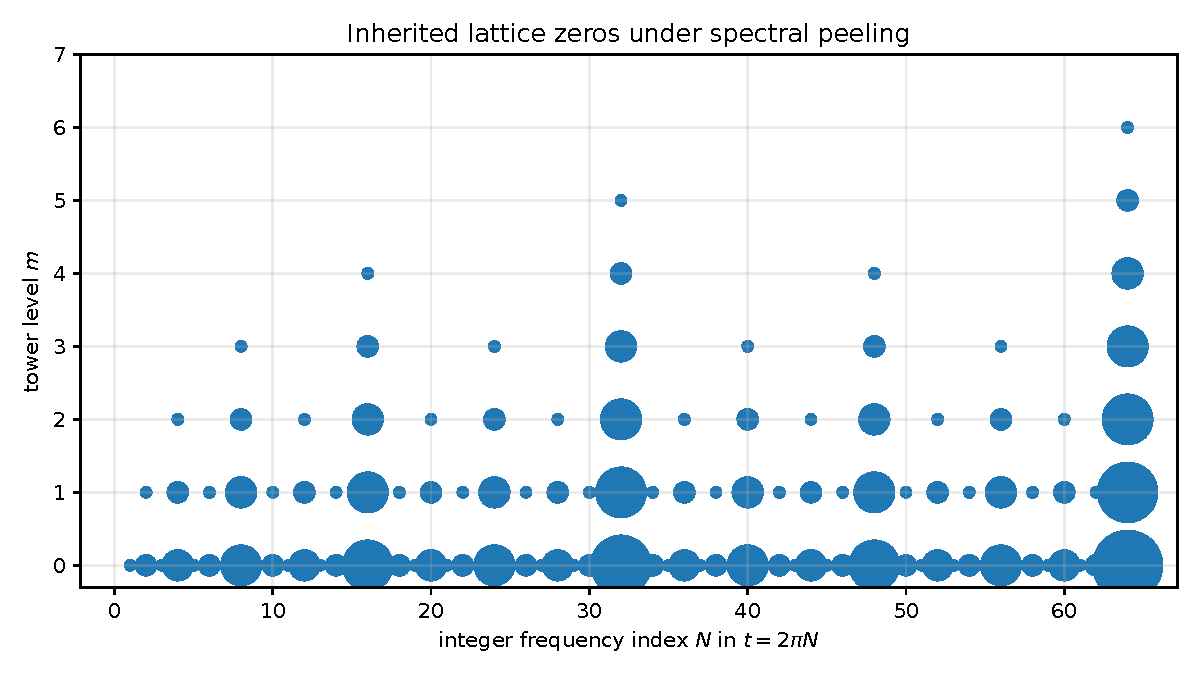
\includegraphics[width=0.95\textwidth]{spectral_peeling.pdf}
\caption{Inherited zero multiplicities for $1\le N\le64$.  Marker area is
proportional to the square of the remaining multiplicity.  Each horizontal
step retains only indices divisible by one additional power of two.}
\label{fig:spectral-peeling}
\end{figure}

\subsection{Integer-base extension}

The same mechanism is not uniquely dyadic.  For an integer $b\ge2$, set
\begin{equation}
 Y_b=\left(1-\frac1b\right)
     \sum_{j=0}^{\infty}b^{-j}U_j.                  \label{eq:Yb}
\end{equation}
At
\begin{equation}
 t_{b,N}=\frac{\pi bN}{b-1},                        \label{eq:tbN}
\end{equation}
the zero multiplicity is $r_b(N)=\nu_b(N)+1$, where $\nu_b(N)$ is the largest
$r$ for which $b^r\mid N$.  If $N=b^{r-1}u$ and
\begin{equation}
 A_{b,u}=\prod_{\ell\ge1}\SincRad(\pi u/b^\ell),
 \qquad
 \varepsilon_{b,N}=(-1)^{u(b^r-1)/(b-1)},           \label{eq:baseb-tail-sign}
\end{equation}
then the first released value is
\begin{equation}
 \phi_{b,r}(t_{b,N})
 =(-1)^r\varepsilon_{b,N}
   \frac{r!(2r-1)!!}{\mu^{(b)}_{2r}t_{b,N}^{2r}}A_{b,u}.       \label{eq:baseb-release}
\end{equation}
Moreover, with $M=\lfloor K/b^m\rfloor$ and $s_b(M)$ the base-$b$ digit sum,
\begin{equation}
 D_{b,m}(K)
 =\frac{bM-s_b(M)}{b-1}.                            \label{eq:baseb-divisor}
\end{equation}
The proof repeats the dyadic argument; the identity
$\sum_{j\ge1}\lfloor M/b^j\rfloor=(M-s_b(M))/(b-1)$ replaces Legendre's
binary formula.

\section{Occupancy calculus and the $q$-Pochhammer layer}
\label{sec:occupancy}

The one-step selector of \Cref{thm:q-selector} is only the first row of a
complete allocation law.  At level $m$, a coordinate may have been zero-biased
more than once.  The resulting collision structure is exactly computable.

\subsection{A general allocation theorem}

Consider first a finite independent symmetric sum
\begin{equation}
 W=X_1+\cdots+X_d,                                  \label{eq:finite-sum}
\end{equation}
and write $\mu_{i,2k}=\Expectation X_i^{2k}$ and
$\mu_{W,2m}=\Expectation W^{2m}$.  Let $X_i^{\langle k\rangle}$ denote the $k$th
zero-bias level of $X_i$.

\begin{theorem}[Zero-bias occupancy law]
\label{thm:occupancy-general}
For every $m\ge0$, choose a weak composition
$\bm k=(k_1,\ldots,k_d)$ of $m$ with probability
\begin{equation}
 \Probability(K_1=k_1,\ldots,K_d=k_d)
 =\frac{(2m-1)!!\,m!}{\mu_{W,2m}}
  \prod_{i=1}^{d}
  \frac{\mu_{i,2k_i}}{k_i!(2k_i-1)!!}.             \label{eq:occupancy-general}
\end{equation}
Conditional on $\bm K$, take all transformed coordinates independently.  Then
\begin{equation}
 W^{\langle m\rangle}
 \stackrel d=\sum_{i=1}^{d}X_i^{\langle K_i\rangle}.             \label{eq:occupancy-mixture}
\end{equation}
The same statement holds for an absolutely summable infinite series by
truncation and weak convergence.
\end{theorem}

\begin{proof}
Let $M_i(t)=\Expectation\EulerE^{tX_i}$ and use the derivation
$\Dop_t=t^{-1}\frac{\Differential}{\Differential t}$.  By
\Cref{thm:radial-derivatives},
\begin{equation}
 \Dop_t^kM_i(t)
 =\frac{\mu_{i,2k}}{(2k-1)!!}
  M_{i,k}(t),                                       \label{eq:component-radial}
\end{equation}
where $M_{i,k}$ is the moment generating function of
$X_i^{\langle k\rangle}$.  Apply the multinomial Leibniz rule to
$\Dop_t^m\prod_iM_i(t)$, then multiply by
$(2m-1)!!/\mu_{W,2m}$.  The coefficients are exactly
\eqref{eq:occupancy-general}; evaluating at $t=0$ proves that they sum to one.
The resulting product of component generating functions proves
\eqref{eq:occupancy-mixture}.
\end{proof}

\subsection{Geometric uniform digits}

For $X_j=c_jU_j$, $c_j=(1-q)q^j$,
\begin{equation}
 \mu_{j,2k}=\frac{c_j^{2k}}{2k+1}.                  \label{eq:uniform-coordinate-moment}
\end{equation}
Thus \eqref{eq:occupancy-general} becomes
\begin{equation}
 \boxed{
 \Probability(\bm K=\bm k)
 =\frac{(2m-1)!!\,m!}{\mu_{2m}(q)}
  \prod_{j\ge0}
  \frac{c_j^{2k_j}}{k_j!(2k_j+1)!!},
 \qquad \sum_jk_j=m.}                              \label{eq:q-occupancy}
\end{equation}
Conditional on $K_j=k$, the $j$th digit is
\begin{equation}
 U_j^{\langle k\rangle}
 \stackrel d=2B_{j,k}-1,
 \qquad B_{j,k}\sim\operatorname{Beta}(k+1,k+1).  \label{eq:uniform-k-tower}
\end{equation}
The local occupancy generating function is the elementary hyperbolic series
\begin{equation}
 \sum_{k=0}^{\infty}\frac{x^k}{k!(2k+1)!!}
 =\frac{\sinh\sqrt{2x}}{\sqrt{2x}}.                \label{eq:local-occupancy-gf}
\end{equation}
Hence the partition function has the exact coefficient form
\begin{equation}
 \frac{\mu_{2m}(q)}{(2m-1)!!\,m!}
 =[z^m]\prod_{j=0}^{\infty}
 \frac{\sinh(c_j\sqrt{2z})}{c_j\sqrt{2z}}.         \label{eq:occupancy-partition}
\end{equation}
This is the positive-coefficient counterpart of the alternating cumulant and
sinc-product expansions.

\begin{theorem}[Collision-free $q$-Pochhammer probability]
\label{thm:collision-free}
The probability that all $m$ zero-bias hits fall on distinct digits is
\begin{equation}
 \boxed{
 \Probability(K_j\in\{0,1\}\ \forall j)
 =\frac{(2m-1)!!\,m!}{\mu_{2m}(q)3^m}
  \frac{(1-q)^{2m}q^{m(m-1)}}{(q^2;q^2)_m}.}        \label{eq:collision-free}
\end{equation}
\end{theorem}

\begin{proof}
Restrict \eqref{eq:q-occupancy} to $k_j\in\{0,1\}$.  The remaining sum is
$3^{-m}$ times the $m$th elementary symmetric function of
$c_0^2,c_1^2,\ldots$.  Euler's identity gives
\begin{equation}
 e_m(1,q^2,q^4,\ldots)
 =\frac{q^{m(m-1)}}{(q^2;q^2)_m}.                  \label{eq:euler-elementary}
\end{equation}
Multiplication by $(1-q)^{2m}$ gives \eqref{eq:collision-free}.
\end{proof}

\begin{table}[ht]
\centering
\caption{Exact collision-free probabilities for the dyadic law $q=1/2$.  A
single step is necessarily collision-free, but repeated hits rapidly
concentrate on the leading digits.}
\label{tab:collision-free}
\small
\begin{tabular}{@{}rll@{}}
\toprule
$m$ & exact probability & decimal \\
\midrule
1 & $1$ & $1$ \\
2 & $10/19$ & $5.2631578947\times10^{-1}$ \\
3 & $70/583$ & $1.2006861063\times10^{-1}$ \\
4 & $1400/132809$ & $1.0541454269\times10^{-2}$ \\
5 & $15400/46840699$ & $3.2877391518\times10^{-4}$ \\
6 & $14014000/4068990560161$ & $3.4440974470\times10^{-6}$ \\
7 & $14014000/1204567303451311$ & $1.1634053124\times10^{-8}$ \\
\bottomrule
\end{tabular}
\end{table}

\subsection{An exact sampler}

Formula \eqref{eq:q-occupancy} gives an efficient sampler even at large tower
levels.  Truncate the digit set after $J$ places, form suffix coefficient tables
for the polynomials
\begin{equation}
 W_j(z)=\sum_{k=0}^{m}\frac{c_j^{2k}}{k!(2k+1)!!}z^k,            \label{eq:Wj}
\end{equation}
and sample each $K_j$ conditionally from the remaining coefficient.  Then draw
the beta digits in \eqref{eq:uniform-k-tower}.  For $q=1/2$ and $J=48$, the
omitted spatial tail is below $4\times10^{-15}$.  The accompanying Python file
implements precisely this dynamic program; it does not use rare-event
rejection from the $2m$-power-biased radius.

\section{Universal Gaussianization}
\label{sec:universal-Gaussian}

The spherical factorization makes the limiting shape nearly universal.
Normalize the endpoint of the support to one.

\begin{theorem}[Universal compact-support Gaussianization]
\label{thm:universal-Gaussian}
Let $W$ be symmetric, nondegenerate, supported in $[-1,1]$, and suppose
\begin{equation}
 \Probability(|W|>1-\varepsilon)>0
 \qquad\text{for every }\varepsilon>0.              \label{eq:endpoint-reached}
\end{equation}
Then
\begin{equation}
 \sqrt{2m}\,W^{\langle m\rangle}
 \ \Longrightarrow\ N(0,1).                       \label{eq:universal-CLT}
\end{equation}
For every fixed $r\ge0$ the moments converge as well:
\begin{equation}
 \Expectation\left[(\sqrt{2m}\,W^{\langle m\rangle})^{2r}\right]
 =(2r-1)!!
  \prod_{j=0}^{r-1}\frac{2m}{2m+2j+1}
  \frac{m_{2m+2r}}{m_{2m}}
 \longrightarrow(2r-1)!!.                          \label{eq:universal-moments}
\end{equation}
\end{theorem}

\begin{proof}
Under the power-biased law \eqref{eq:power-radius}, for every
$\varepsilon>0$,
\[
 \Probability(R_m\le1-\varepsilon)
 =\frac{\Expectation[|W|^{2m}\mathbf 1_{\{|W|\le1-\varepsilon\}}]}{m_{2m}}
 \longrightarrow0.
\]
Indeed, compare the numerator with a fixed positive amount of mass in
$|W|>1-\varepsilon/2$.  Thus $R_m\to1$ in probability.

The spherical representation gives
\[
 B_m\stackrel d=
 \frac{G_1}{(G_1^2+\cdots+G_{2m+1}^2)^{1/2}},
\qquad G_j\stackrel{\mathrm{iid}}\sim N(0,1).
\]
Hence $\sqrt{2m}B_m\Rightarrow N(0,1)$ by the law of large numbers.  Slutsky's
theorem and \eqref{eq:spherical-factorization} prove
\eqref{eq:universal-CLT}.  Formula \eqref{eq:universal-moments} is
\eqref{eq:tower-moment-formula} after scaling.  The tilted radius concentrates
at one, so $m_{2m+2r}/m_{2m}\to1$.
\end{proof}

\begin{corollary}[Escape of characteristic zeros]
Let $\tau_m$ be the smallest positive zero of the Rvachev tower characteristic
function $\phi_m$.  Then
\begin{equation}
 \frac{\tau_m}{\sqrt{2m}}\longrightarrow\infty.     \label{eq:zero-escape}
\end{equation}
\end{corollary}

\begin{proof}
The characteristic functions of
$\sqrt{2m}\Tower{m}$ converge uniformly on compact sets to
$\EulerE^{-t^2/2}$, which has no real zero.  Corollary \ref{cor:LP-hierarchy}
ensures that $\tau_m$ is a real zero, so it must leave every compact scaled
interval.
\end{proof}

The theorem gives convergence but no rate.  For ordinary endpoint densities,
$1-R_m$ is typically of order $1/m$.  The Rvachev density is infinitely flat at
the endpoint, and this changes the scale to $(\log m)/m$.  The next section
makes that statement exact.

\section{Fabius endpoint bias and phase-modulated mod-Gamma asymptotics}
\label{sec:mod-gamma}

\subsection{A bridge from absolute moments to the Fabius law}

The endpoint radius is governed by the same negative-Laplace product that
controls the small-argument Fabius asymptotics.

\begin{lemma}[Moment--CDF bridge]
\label{lem:moment-bridge}
For every real $a>-1$,
\begin{equation}
 \boxed{
 \mu_a=\Expectation|Y|^a
 =\frac{2}{a+1}\Expectation X^{a+1}.}                         \label{eq:moment-CDF-bridge}
\end{equation}
\end{lemma}

\begin{proof}
Using \eqref{eq:up-F}, reflection of $X$, and Stieltjes integration by parts,
\begin{align*}
 \mu_a
 &=2\int_0^1r^aF(1-r)\Differential r
  =2\int_0^1(1-x)^aF(x)\Differential x\\
 &=\frac{2}{a+1}\Expectation(1-X)^{a+1}
  =\frac{2}{a+1}\Expectation X^{a+1}.
\end{align*}
\end{proof}

For $n>0$, let $\mathcal R_n$ denote the $n$-power-biased radius:
\begin{equation}
 \Expectation g(\mathcal R_n)
 =\frac{\Expectation[|Y|^ng(|Y|)]}{\mu_n}.                   \label{eq:Rn-general}
\end{equation}
Thus the radius in the level-$m$ factorization is
$R_m=\mathcal R_{2m}$.  Put
\begin{equation}
 T_n=n(1-\mathcal R_n).                             \label{eq:Tn}
\end{equation}
After the change of variable $x=1-r$, the Laplace transform of $T_n$ is
\begin{equation}
 \Expectation\EulerE^{-uT_n}
 =\frac{I_n(u)}{I_n(0)},
 \qquad
 I_n(u)=\int_0^1\EulerE^{-unx}(1-x)^nF(x)\Differential x.          \label{eq:In}
\end{equation}
The auxiliary Laplace integral
\begin{equation}
 J(s)=\int_0^1\EulerE^{-sx}F(x)\Differential x
 =\frac{L_X(s)-\EulerE^{-s}}{s}                         \label{eq:J-L}
\end{equation}
follows by integration by parts.

\begin{lemma}[Power tilt versus exponential tilt]
\label{lem:power-laplace}
Uniformly for $u$ in a fixed compact subset of $(-1,\infty)$,
\begin{equation}
 \frac{I_n(u)}{I_n(0)}
 =\frac{J((1+u)n)}{J(n)}
  \left(1+\BigO\!\left(\frac{(\log n)^2}{n}\right)\right).     \label{eq:power-laplace}
\end{equation}
The same estimate remains valid after any fixed number of derivatives with
respect to $u$ in a neighborhood of the origin.
\end{lemma}

\begin{proofidea}
The inequality $\log(1-x)\le-x$ gives $(1-x)^n\le\EulerE^{-nx}$.  On
$0\le x\le1/2$,
\[
 0\le \EulerE^{-nx}-(1-x)^n
 \le Cnx^2\EulerE^{-nx}.
\]
For the measure proportional to $\EulerE^{-sx}F(x)\Differential x$, derivatives of
\eqref{eq:Lambda} and \eqref{eq:J-L} give
\[
 \Expectation_s x^k=\BigO_k\!\left((\log s/s)^k\right).
\]
Consequently, the relative error made by replacing $(1-x)^n$ with
$\EulerE^{-nx}$ is $O((\log n)^2/n)$.  The region $x>1/2$ is exponentially small
relative to $J(n)$, whose logarithm has only quadratic-logarithmic decay.
Inserting fixed powers of $nx$ proves the differentiated estimates.
\end{proofidea}

\subsection{A periodic mod-Gamma law}

Define
\begin{equation}
 \alpha_n=\log_2n+\frac12,
 \qquad \theta_n=\log_2n,                           \label{eq:alpha-theta}
\end{equation}
and, for $u>-1$,
\begin{equation}
 \mathcal R_\theta(u)
 =\exp\!\left[
   -\frac{\log^2(1+u)}{2L}
   +\Psi\!\left(\theta+\log_2(1+u)\right)-\Psi(\theta)
  \right].                                         \label{eq:modgamma-residue}
\end{equation}
The notation $\mathcal R_\theta$ here denotes the residue function, not the
power-biased radius $\mathcal R_n$; the distinction is always clear from the
argument.

\begin{theorem}[Phase-modulated mod-Gamma endpoint law]
\label{thm:mod-gamma}
Uniformly for $u$ in a fixed compact subset of $(-1,\infty)$,
\begin{equation}
 \boxed{
 \Expectation\EulerE^{-uT_n}
 =(1+u)^{-\alpha_n}\mathcal R_{\theta_n}(u)
  \left(1+\BigO\!\left(\frac{(\log n)^2}{n}\right)\right).}    \label{eq:modgamma-main}
\end{equation}
In particular, along every sequence for which the fractional part of
$\log_2n$ tends to $\theta$,
\begin{equation}
 (1+u)^{\alpha_n}\Expectation\EulerE^{-uT_n}
 \longrightarrow\mathcal R_\theta(u).              \label{eq:modgamma-subsequence}
\end{equation}
\end{theorem}

\begin{proof}
By \Cref{lem:power-laplace} and \eqref{eq:J-L}, the logarithm of the left side
is
\[
 \Lambda((1+u)n)-\Lambda(n)-\log(1+u)
 +\BigO((\log n)^2/n).
\]
Put $a=\log(1+u)$.  Substituting \eqref{eq:Lambda} gives
\begin{align*}
 &-\frac{(\log n+a)^2-(\log n)^2}{2L}
   +\frac a2-a
   +\Psi(\theta_n+a/L)-\Psi(\theta_n)\\
 &\qquad
 =-\left(\frac{\log n}{L}+\frac12\right)a
   -\frac{a^2}{2L}
   +\Psi(\theta_n+\log_2(1+u))-\Psi(\theta_n).
\end{align*}
Exponentiation proves \eqref{eq:modgamma-main}.
\end{proof}

The dominant factor $(1+u)^{-\alpha_n}$ is the Laplace transform of a
Gamma$(\alpha_n,1)$ variable.  The Gamma--zeta periodic function survives as a
bounded phase cocycle rather than disappearing in the limit.

\begin{corollary}[Endpoint mean, variance, and central limit theorem]
\label{cor:endpoint-cumulants}
As $n\to\infty$,
\begin{align}
 \Expectation T_n
 &=\alpha_n-\frac{\Psi'(\theta_n)}{L}
   +\BigO\!\left(\frac{(\log n)^2}{n}\right),        \label{eq:Tn-mean}\\
 \Variance(T_n)
 &=\alpha_n-\frac1L
   -\frac{\Psi'(\theta_n)}{L}
   +\frac{\Psi''(\theta_n)}{L^2}
   +\BigO\!\left(\frac{(\log n)^2}{n}\right).      \label{eq:Tn-var}
\end{align}
Moreover,
\begin{equation}
 \frac{T_n-\bigl(\alpha_n-\Psi'(\theta_n)/L\bigr)}
      {\sqrt{\alpha_n}}
 \Longrightarrow N(0,1).                           \label{eq:Tn-CLT}
\end{equation}
\end{corollary}

\begin{proof}
Differentiate the logarithm of \eqref{eq:modgamma-main} at $u=0$.  The first
two derivatives of $a=\log(1+u)$ are $1$ and $-1$, which gives
\eqref{eq:Tn-mean} and \eqref{eq:Tn-var}.  For
\eqref{eq:Tn-CLT}, evaluate the moment generating function at an argument of
order $\alpha_n^{-1/2}$ and expand $\log(1+u)$.  The residue contributes only
bounded cumulants, while the Gamma factor contributes $\alpha_n$ to every
fixed cumulant before standardization.
\end{proof}

\begin{figure}[ht]
\centering
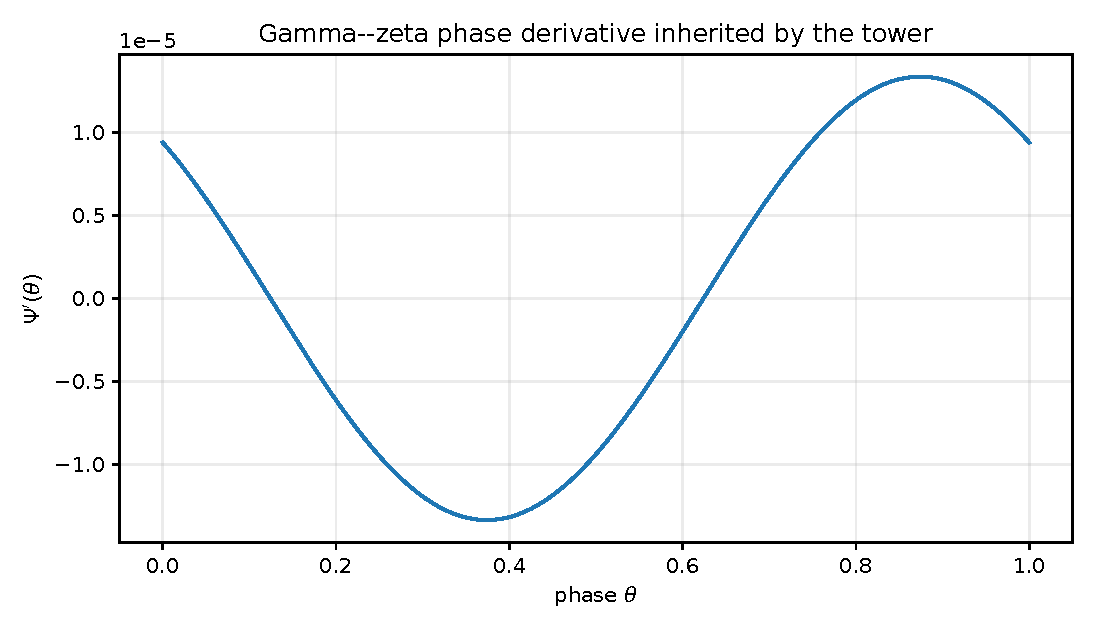
\includegraphics[width=0.88\textwidth]{periodic_phase_derivative.pdf}
\caption{The periodic derivative $\Psi'$ computed from
\eqref{eq:Psi-Fourier}.  Its amplitude is only about $1.4\times10^{-5}$, but it
enters the exact first phase-resolved term of the endpoint mean and every fixed
moment ratio.}
\label{fig:periodic-derivative}
\end{figure}

\subsection{High-moment and tower-moment consequences}

Since
\(
 \Expectation\mathcal R_n^k=\mu_{n+k}/\mu_n
\), the endpoint law immediately gives fixed-shift moment ratios.

\begin{corollary}[Phase-resolved high-moment ratios]
\label{cor:high-moment-ratio}
For every fixed positive integer $k$,
\begin{equation}
 \boxed{
 1-\frac{\mu_{n+k}}{\mu_n}
 =\frac{k}{n}
  \left(
    \log_2n+\frac12-\frac{\Psi'(\log_2n)}{L}
  \right)
 +\BigO_k\!\left(\frac{(\log n)^2}{n^2}\right).}    \label{eq:high-moment-ratio}
\end{equation}
In particular,
\begin{equation}
 1-\frac{\mu_{2m+2}}{\mu_{2m}}
 \sim\frac{\log(2m)}{m\log2}.                      \label{eq:even-ratio-leading}
\end{equation}
\end{corollary}

\begin{proof}
Write $\mathcal R_n=1-T_n/n$ and expand
$1-(1-T_n/n)^k$.  By \eqref{eq:Tn-mean}, the linear term gives the displayed
coefficient.  The second moment is $O((\log n)^2)$ by
\eqref{eq:Tn-var}, so all remaining terms contribute
$O_k((\log n)^2/n^2)$.
\end{proof}

Combining \eqref{eq:high-moment-ratio} with
\eqref{eq:universal-moments} gives a phase-resolved rate for every fixed tower
moment.

\begin{corollary}[First correction to Gaussian tower moments]
\label{cor:tower-moment-correction}
Put $n=2m$.  For fixed $r\ge1$,
\begin{align}
 &\frac{\Expectation[(\sqrt{2m}\Tower{m})^{2r}]}{(2r-1)!!}
 \notag\\
 &\quad=1-
 \frac{
   2r\log_2n+r+r^2-2r\Psi'(\log_2n)/L
 }{n}
 +\BigO_r\!\left(\frac{(\log n)^2}{n^2}\right).    \label{eq:tower-moment-correction}
\end{align}
For the variance this specializes to
\begin{equation}
 1-\Variance(\sqrt{2m}\Tower{m})
 =\frac{2\log_2(2m)+2-2\Psi'(\log_2(2m))/L}{2m}
 +\BigO\!\left(\frac{(\log m)^2}{m^2}\right).       \label{eq:tower-variance-correction}
\end{equation}
\end{corollary}

\begin{proof}
For fixed $r$, \eqref{eq:high-moment-ratio} gives
\[
 \frac{\mu_{n+2r}}{\mu_n}
 =1-\frac{2r}{n}
   \left(\log_2n+\frac12-\frac{\Psi'(\log_2n)}L\right)
   +O_r((\log n)^2/n^2).
\]
The universal beta factor satisfies
\[
 \prod_{j=0}^{r-1}\frac{n}{n+2j+1}
 =1-\frac{r^2}{n}+O_r(n^{-2}).
\]
Multiplying proves the claim.
\end{proof}

\begin{figure}[ht]
\centering
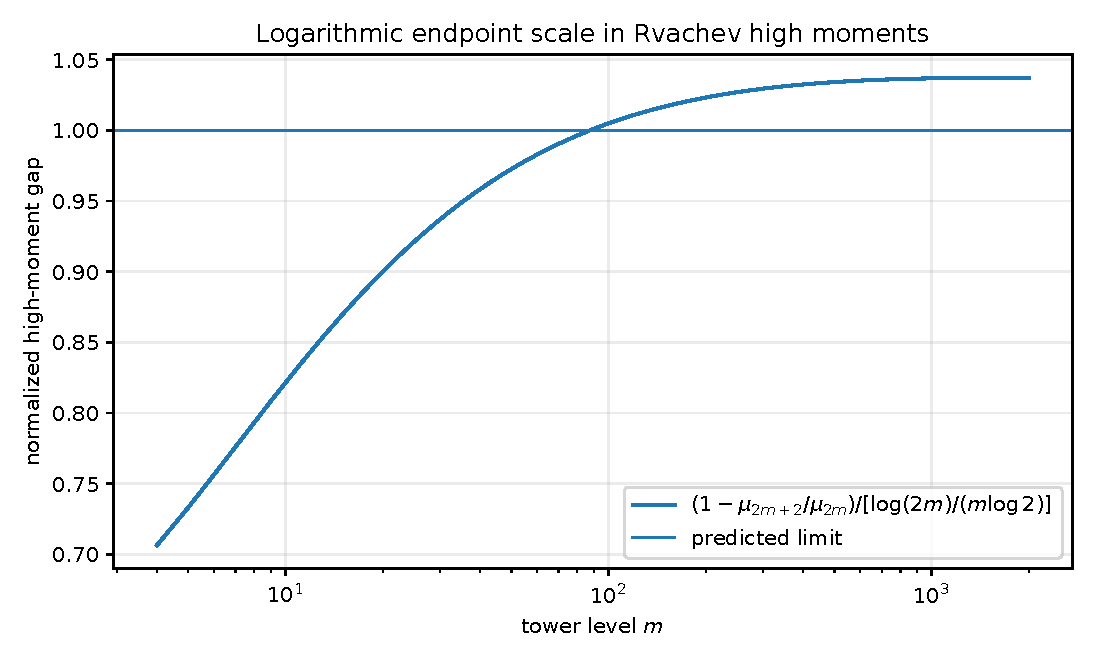
\includegraphics[width=0.9\textwidth]{moment_ratio_convergence.pdf}
\caption{The normalized gap in \eqref{eq:even-ratio-leading}, computed by the
positive moment recurrence in \Cref{app:numerics}.  The slow drift above one is
consistent with the explicit constant term in
\eqref{eq:high-moment-ratio}; the periodic term is much smaller on this scale.}
\label{fig:moment-ratio}
\end{figure}

\begin{figure}[ht]
\centering
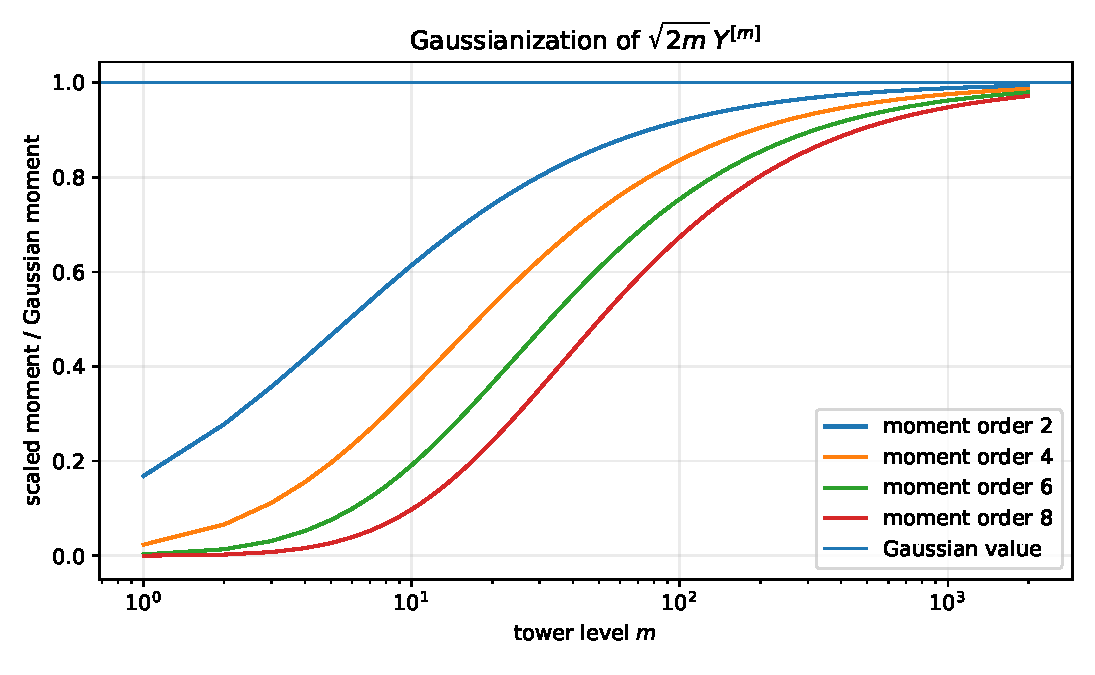
\includegraphics[width=0.9\textwidth]{tower_moment_convergence.pdf}
\caption{The first four even moments of $\sqrt{2m}\Tower{m}$, divided by their
Gaussian values.  Higher moments converge more slowly, as predicted by the
factor $2r\log_2(2m)/(2m)$ in
\eqref{eq:tower-moment-correction}.}
\label{fig:tower-moments}
\end{figure}

\subsection{A sharp leading Wasserstein rate}

Let $Z\sim N(0,1)$ and set
\begin{equation}
 Z_m=\sqrt{2m}\Tower{m},
 \qquad G_m=\sqrt{2m}B_m.                           \label{eq:Zm-Gm}
\end{equation}
The factorization couples $Z_m=R_mG_m$ with $R_m$ independent of $G_m$.

\begin{lemma}[Spherical-coordinate normal approximation]
\label{lem:beta-W1}
For the beta coordinate in \eqref{eq:Bm-density},
\begin{equation}
 W_1(G_m,Z)=\BigO(m^{-1}).                           \label{eq:beta-W1}
\end{equation}
Moreover,
\begin{equation}
 \Expectation|G_m|
 =\sqrt{2m}\frac{c_m}{m}
 =\sqrt{\frac2\pi}\left(1-\frac1{8m}+O(m^{-2})\right).         \label{eq:Gm-abs}
\end{equation}
\end{lemma}

\begin{proofidea}
The density of $G_m$ is
\[
 g_m(x)=\frac{c_m}{\sqrt{2m}}
 \left(1-\frac{x^2}{2m}\right)_{+}^{m-1}.
\]
Stirling's expansion for $c_m$ and a Taylor expansion of the logarithm show
that the first absolute moment of the signed density difference from the
standard normal is $O(1/m)$; this bounds $W_1$.  The exact integral
$\Expectation|B_m|=c_m/m$ gives \eqref{eq:Gm-abs}.
\end{proofidea}

\begin{theorem}[Sharp leading transport scale]
\label{thm:W1-rate}
For the Rvachev zero-bias tower,
\begin{equation}
 \boxed{
 W_1(Z_m,Z)
 \sim \sqrt{\frac2\pi}\,
       \frac{\log(2m)}{2m\log2}.}                   \label{eq:W1-rate}
\end{equation}
\end{theorem}

\begin{proof}
Let
\[
 d_m=\Expectation(1-R_m)=1-\frac{\mu_{2m+1}}{\mu_{2m}}.
\]
By \eqref{eq:high-moment-ratio},
\begin{equation}
 d_m
 =\frac{\log_2(2m)+1/2-\Psi'(\log_2(2m))/L}{2m}
  +O((\log m)^2/m^2).                               \label{eq:dm}
\end{equation}
The factorization coupling gives
\[
 W_1(Z_m,G_m)
 \le\Expectation|G_m|(1-R_m)=\Expectation|G_m|d_m.
\]
Together with \Cref{lem:beta-W1}, this yields
\begin{equation}
 W_1(Z_m,Z)
 \le\sqrt{\frac2\pi}d_m+O(m^{-1}).                 \label{eq:W1-upper}
\end{equation}
For the reverse bound, the function $x\mapsto|x|$ is $1$-Lipschitz, so
\begin{align*}
 W_1(Z_m,Z)
 &\ge \Expectation|Z|-\Expectation|Z_m|\\
 &=\sqrt{\frac2\pi}-\Expectation|G_m|\Expectation R_m
  =\sqrt{\frac2\pi}d_m+O(m^{-1}).                  \label{eq:W1-lower}
\end{align*}
Since $d_m\sim\log(2m)/(2m\log2)$ dominates $m^{-1}$, the upper and lower
bounds have the same leading term.
\end{proof}

\begin{remark}[Where Lambert $W$ went]
The inverse Fabius endpoint problem uses a lower-Lambert variable because one
must invert the relation between a tiny probability and its saddle scale.  In
the high-moment problem the saddle parameter is already supplied externally:
it is the moment order $n$.  The same quadratic logarithm and the same
Gamma--zeta phase therefore appear directly at $\log_2n$, without an additional
Lambert inversion.  In this precise sense the tower is the
\emph{deparametrized Laplace-side companion} of the lower-$W_{-1}$ endpoint
asymptotics.
\end{remark}

\section{Numerical experiments}
\label{sec:numerics}

The accompanying program
\path{zero_bias_tower_experiments.py} performs both exact and floating-point
checks.  It uses no external data.  Its principal computations are:
\begin{enumerate}
\item exact rational moments from Bernoulli cumulants and the complete Bell
      recurrence;
\item a positive, cancellation-free moment recurrence derived from
      $Y\stackrel d=(Y+U)/2$;
\item exact collision probabilities and release signs;
\item evaluation of $\Psi'$ from the exponentially convergent Gamma--zeta
      Fourier series;
\item occupancy-based Monte Carlo sampling of tower densities;
\item deterministic moment and spectral-peeling plots.
\end{enumerate}
The repository intake replay pins the five Python dependencies listed in
\path{requirements.txt}.  The exact moment, collision, and released-Fourier
tables reproduce the delivered bytes.  Three floating-point tables differ
only in last-place rounding across the updated numerical stack (maximum
absolute difference $7.31\times10^{-14}$); figure geometry and mathematical
content are unchanged, while antialiasing and vector-font encoding are
platform dependent.  These observations are reproducibility evidence only,
not formal proofs of the manuscript theorems.

\subsection{Selected high-moment data}

\begin{table}[ht]
\centering
\caption{Even-moment ratios and the variance of the scaled tower.}
\label{tab:moment-data}
\small
\begin{tabular}{@{}rrrr@{}}
\toprule
$m$ & $\mu_{2m+2}/\mu_{2m}$
& normalized gap in \eqref{eq:even-ratio-leading}
& $\Variance(\sqrt{2m}\Tower{m})$ \\
\midrule
10   & 0.644909548417 & 0.821601942 & 0.614199569921 \\
20   & 0.760481812449 & 0.900118090 & 0.741933475560 \\
50   & 0.870759209336 & 0.972633866 & 0.862137831026 \\
100  & 0.923183207674 & 1.004948163 & 0.918590256392 \\
200  & 0.955776340501 & 1.023239131 & 0.953392858355 \\
500  & 0.979388268891 & 1.034124888 & 0.978409859032 \\
1000 & 0.988631011017 & 1.036769344 & 0.988136942545 \\
1500 & 0.992013838782 & 1.037096739 & 0.991683277689 \\
\bottomrule
\end{tabular}
\end{table}

The normalized gap need not approach one monotonically.  The $1/n$ constant
term is still visible when divided by the leading $(\log n)/n$ term, and the
phase correction is roughly five orders of magnitude smaller than unity.

\subsection{Occupancy sampling}

\begin{figure}[ht]
\centering
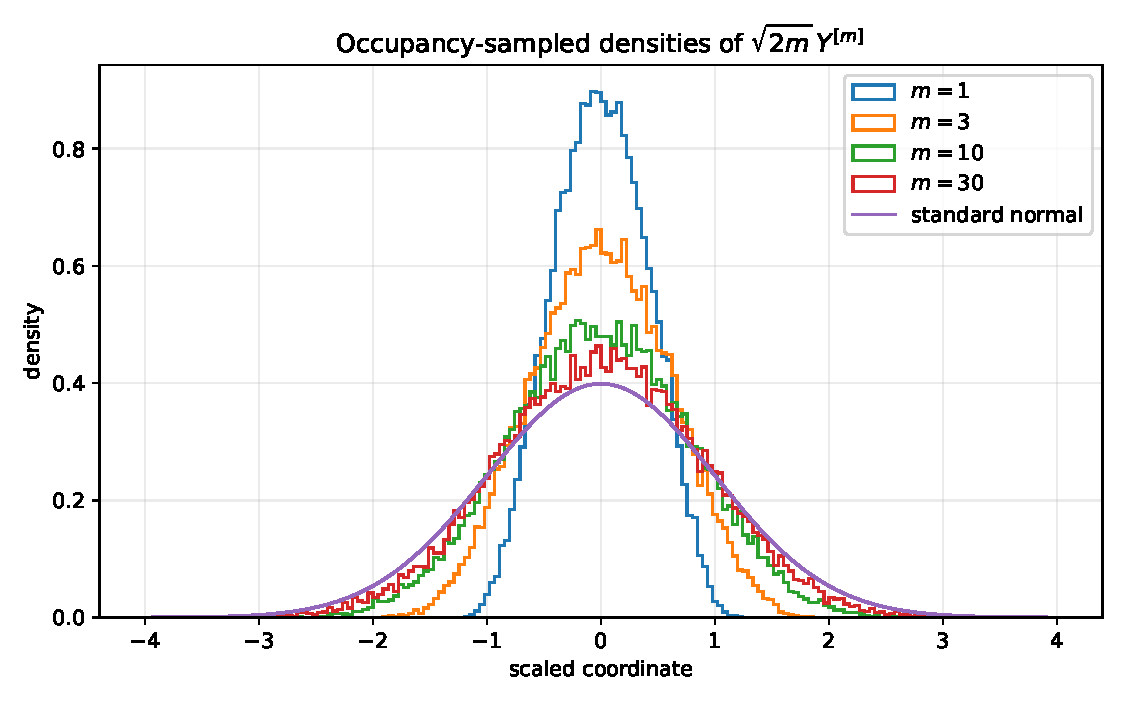
\includegraphics[width=0.92\textwidth]{tower_density_monte_carlo.pdf}
\caption{Occupancy-sampled densities of $\sqrt{2m}\Tower{m}$ compared with the
standard normal density.  The plots use the exact conditional beta digits from
\eqref{eq:uniform-k-tower}; no endpoint rejection sampling is involved.}
\label{fig:tower-density}
\end{figure}

The variance check written by the script compares Monte Carlo estimates with
\eqref{eq:tower-variance}.  Because the displayed normalization is
$\sqrt{2m}$ rather than exact unit variance, the low-level curves are visibly
narrower than the normal.  This is predicted quantitatively by
\eqref{eq:tower-variance-correction}, not a sampling defect.

\section{Conjectures and frontier problems}
\label{sec:conjectures}

The exact results above expose several problems that are both structurally
natural and sufficiently constrained to support serious attack.

\begin{conjecture}[No spectral reappearance]
\label{conj:no-reappearance}
Let $N\ge1$ and $r=\nu_2(N)+1$.  Then
\begin{equation}
 \phi_m(2\pi N)\ne0\qquad\text{for every }m\ge r.   \label{eq:no-reappearance}
\end{equation}
Equivalently, once the inherited lattice zero has been released at level $r$,
it never reappears as an accidental zero of a later normalized derivative of
$H$.
\end{conjecture}

The statement is stronger than ordinary interlacing.  Writing
$H(z)=(1+z/(\pi^2N^2))^rQ_N(z)$ reduces it to the nonvanishing of
$Q_N^{(m-r)}(-\pi^2N^2)$.  Total positivity may impose a sign regularity on
these derivatives that is invisible in the unnormalized product.

\begin{conjecture}[Bessel--Airy first-zero transition]
\label{conj:Bessel-Airy}
Let $\tau_{m,k}$ be the $k$th positive zero of $\phi_m$, and let
$j_{m-1/2,k}$ be the $k$th positive zero of $J_{m-1/2}$.  For fixed $k$,
\begin{equation}
 \tau_{m,k}
 =j_{m-1/2,k}
  +\frac12\left(
      \log_2(2m)+\frac12-\frac{\Psi'(\log_2(2m))}{L}
    \right)
  +o(1).                                            \label{eq:Bessel-Airy}
\end{equation}
\end{conjecture}

The first term is forced by the spherical beta factor.  At the Bessel turning
point, fluctuations of $R_m$ occur on a scale much smaller than the
$m^{1/3}$ Airy scale, while the mean contraction shifts the argument by
approximately $j_{m-1/2,k}\Expectation(1-R_m)$.  A proof should combine uniform turning
point asymptotics for Bessel functions with the mod-Gamma law of
\Cref{thm:mod-gamma}.

\begin{conjecture}[Geometric occupancy limit shape]
\label{conj:occupancy-shape}
For fixed $q\in(0,1)$ and $c_j=(1-q)q^j$, let $K_j^{(m)}$ have the occupancy law
\eqref{eq:q-occupancy}.  Then, for each fixed $J$,
\begin{equation}
 \left(\frac{K_0^{(m)}}m,\ldots,\frac{K_J^{(m)}}m\right)
 \longrightarrow(c_0,\ldots,c_J)                  \label{eq:occupancy-LLN}
\end{equation}
in probability.  After centering and scaling by $\sqrt m$, the finite vectors
converge to a Gaussian law with covariance
\begin{equation}
 \frac12\bigl(c_i\delta_{ij}-c_ic_j\bigr)_{0\le i,j\le J}.      \label{eq:occupancy-CLT}
\end{equation}
\end{conjecture}

A saddle parameter $z\sim2m^2$ in the product
\eqref{eq:occupancy-partition} predicts
\(
 \Expectation K_j\sim c_jm
\)
and grand-canonical variance $c_jm/2$.  Conditioning on the total occupancy
produces the rank-one covariance correction in \eqref{eq:occupancy-CLT}.
Multivariate analytic combinatorics should make this route rigorous.

\begin{conjecture}[All-order phase-resolved Gaussianization]
\label{conj:all-order-Gaussian}
For every fixed $r$, the ratio in
\eqref{eq:tower-moment-correction} admits a complete expansion
\begin{equation}
 \frac{\Expectation[(\sqrt{2m}\Tower{m})^{2r}]}{(2r-1)!!}
 \sim1+\sum_{j\ge1}\frac{P_{r,j}(\log m,\{\log_2m\})}{m^j},    \label{eq:all-order-Gaussian}
\end{equation}
where $P_{r,j}$ is polynomial in $\log m$ and smooth periodic in the dyadic
phase.  Its periodic coefficients are differential polynomials in $\Psi$.
An analogous expansion holds for smooth test functions against the Gaussian
law.
\end{conjecture}

The exact decomposition \eqref{eq:Lambda}, the power-to-Laplace replacement,
and Bell-polynomial differentiation make this conjecture highly structured.
The main work is uniform bookkeeping rather than discovery of new saddle
points.

\begin{conjecture}[Monotone standardized Stein discrepancy]
\label{conj:Stein-monotone}
Let $\widetilde Y_m=\Tower{m}/\sqrt{\Variance(\Tower{m})}$.  A natural quadratic
Stein discrepancy, and possibly the relative entropy to the standard normal,
is eventually strictly decreasing in $m$.
\end{conjecture}

Zero bias fixes the normal distribution after variance normalization, and the
tower is an explicit deterministic orbit toward that fixed point.  The
spherical factorization and the density descent
\eqref{eq:density-descent} provide unusually concrete tools for testing
contractivity.

\subsection{Further directions}

\paragraph{Integer and nonintegral geometric bases.}
The release formula \eqref{eq:baseb-release} and divisor count
\eqref{eq:baseb-divisor} should be combined with the arbitrary-base
negative-Laplace decomposition.  For integer $b$, one expects a
$\log_b n$-periodic mod-Gamma residue and a base-$b$ digit-sign release law.
For general $q$, the occupancy theorem is already exact; Mellin analysis should
supply the corresponding period $\log(1/q)$.

\paragraph{Ultraspherical and Legendre synthesis.}
The kernel $(1-u^2)^{m-1}$ is the Gegenbauer weight with parameter
$m-1/2$.  Thus the tower defines a triangular transform from the repository's
Legendre coefficients of $\RvachevUp$ to ultraspherical coefficients of $p_m$.  An
explicit coefficient map could close a new representation loop and may be
better conditioned than repeated differentiation of the Legendre series.

\paragraph{Dyadic exact values.}
Formula \eqref{eq:density-kernel} expands into finitely many weighted
primitives of $\RvachevUp$.  At dyadic $x$, the repository's exact primitive and
moment machinery should therefore yield rational values of $p_m(x)$ and its
derivatives.  Determining denominator valuations as a function of $(m,x)$ is a
concrete arithmetic project.

\paragraph{Multivariate masks.}
For compactly supported refinable densities generated by vector-valued uniform
series, directional zero bias should replace a variance-weighted coordinate
and produce a spherical factor in the chosen direction.  The analogue of
spectral peeling would act on hyperplane zero arrangements of the Fourier
mask.

\section{Lean formalization plan}
\label{sec:lean-plan}

The new results divide naturally into small reusable modules.  A practical
formalization order is:
\begin{enumerate}
\item define zero bias for symmetric compactly supported probability measures
      through the test-function identity and prove the polynomial moment rule
      \eqref{eq:zero-bias-moments};
\item formalize the independent-sum replacement theorem and specialize it to
      the $q^2$-geometric selector \eqref{eq:J-law};
\item define the symmetric tower and prove the moment formula
      \eqref{eq:tower-moment-formula};
\item construct the beta coordinate $B_m$, prove its even moments, and identify
      the product law $R_mB_m$ by compact moment determinacy;
\item prove the radial derivative identities and connect them to the existing
      entire transform $H$;
\item reuse the current zero-multiplicity and Thue--Morse sign theorems to prove
      \eqref{eq:released-value} and \eqref{eq:Dm-formula};
\item formalize the finite occupancy theorem with formal power series, then
      pass to the geometric infinite series by the repository's existing
      truncation infrastructure;
\item import the negative-Laplace decomposition to establish the leading
      endpoint mean, high-moment ratio, and Wasserstein asymptotic.
\end{enumerate}
The first six items require little asymptotic infrastructure and are plausible
near-term targets.  The mod-Gamma theorem needs a small library for uniform
Laplace-tilt moment bounds, but its analytic input is already present in the
formal development.

\section{Conclusion}

The zero-bias transform reveals a coherent layer that was not explicit in the
inspected Fabius--Rvachev corpus.  It turns the derivatives of the
Laguerre--P\'olya transform into genuine probability laws; it converts the
geometric random series into a $q^2$-selected digit replacement process; it
organizes repeated replacements by a positive occupancy partition function;
and it differentiates the arithmetic Fourier divisor one order at a time.
The first value released from a multiple zero remembers the odd tail of the
sinc product and hence the Thue--Morse sign.

At large depth, a universal spherical coordinate forces Gaussian shape.  The
Fabius endpoint nevertheless leaves a precise fingerprint: a power-biased
radius with Gamma-scale fluctuations of size $\log_2m$, a nonconstant
Gamma--zeta phase residue, and a Wasserstein delay of order $(\log m)/m$.
This connects the probability, q-series, entire-function, Fourier-arithmetic,
and Lambert-asymptotic parts of the repository without duplicating their
existing central theorems.

\appendix

\section{Stable moment recurrence and exact checks}
\label{app:numerics}

The cumulant recurrence from \eqref{eq:cumulants} is exact but alternating.
For high degrees, the distributional fixed point
\begin{equation}
 Y\stackrel d=\frac{Y'+U}{2}                        \label{eq:Y-fixed-point}
\end{equation}
provides a positive recurrence.  Taking the $2r$th moment and isolating the
self-term gives
\begin{equation}
 \boxed{
 \mu_{2r}
 =\frac{1}{2^{2r}-1}
  \sum_{j=0}^{r-1}
  \binom{2r}{2j}\frac{\mu_{2j}}{2r-2j+1}.}          \label{eq:positive-moment-recurrence}
\end{equation}
Every summand is nonnegative.  Evaluating the normalized binomial weights via
log-Gamma functions makes the recurrence stable in ordinary double precision
through at least the several thousand moments needed by the figures.

For low degrees, the exact values generated by the Bell recurrence begin
\begin{align*}
 \mu_0&=1,&
 \mu_2&=\frac19,&
 \mu_4&=\frac{19}{675},\\
 \mu_6&=\frac{583}{59535},&
 \mu_8&=\frac{132809}{32531625},&
 \mu_{10}&=\frac{46840699}{24405225075}.
\end{align*}
These values independently normalize the released-value and collision tables.

\section{Occupancy dynamic program}
\label{app:occupancy-DP}

For a fixed tower level $m$, truncate after $J$ geometric digits and define
\begin{equation}
 w_j(k)=\frac{c_j^{2k}}{k!(2k+1)!!},
 \qquad 0\le k\le m.                                \label{eq:wjk}
\end{equation}
Let $S(j,r)$ be the coefficient of $z^r$ in
$\prod_{\ell=j}^{J-1}\sum_{k=0}^mw_\ell(k)z^k$.  Backward convolution computes
all $S(j,r)$ in $O(Jm^2)$ operations.  Given that $r$ hits remain at digit $j$,
choose $k$ with probability
\begin{equation}
 \Probability(K_j=k\mid r\text{ remain})
 =\frac{w_j(k)S(j+1,r-k)}{S(j,r)}.                  \label{eq:DP-transition}
\end{equation}
After the occupancy vector is sampled, draw the independent beta digits from
\eqref{eq:uniform-k-tower}.  The recurrence
\begin{equation}
 \frac{w_j(k)}{w_j(k-1)}
 =\frac{c_j^2}{k(2k+1)}                             \label{eq:wj-recurrence}
\end{equation}
avoids factorial overflow.

\section{Files generated by the companion program}

A default run writes:
\begin{itemize}
\item \path{data/exact_even_moments.csv};
\item \path{data/high_moment_ratios.csv};
\item \path{data/collision_free_probabilities.csv};
\item \path{data/released_fourier_values.csv};
\item \path{data/tower_moment_convergence.csv};
\item \path{data/occupancy_sampler_checks.csv};
\item the PDF and PNG versions of all figures used in this report.
\end{itemize}
The source is extensively commented and accepts command-line options for the
maximum moment degree, Monte Carlo sample count, and random seed.

\begin{thebibliography}{99}

\bibitem{arias1982}
J.~Arias de Reyna,
\newblock A function of Rvachev,
\newblock original Spanish article (1982); English translation,
\emph{arXiv:1702.05442}, 2017.

\bibitem{arias2018}
J.~Arias de Reyna,
\newblock Arithmetic of the Fabius function,
\newblock \emph{arXiv:1702.06487}, revised 2018.

\bibitem{corless1996}
R.~M. Corless, G.~H. Gonnet, D.~E.~G. Hare, D.~J. Jeffrey, and D.~E. Knuth,
\newblock On the Lambert $W$ function,
\newblock \emph{Advances in Computational Mathematics} \textbf{5} (1996),
329--359.

\bibitem{dobler2015}
C.~D\"obler,
\newblock Distributional transformations without orthogonality relations,
\newblock \emph{Journal of Theoretical Probability} \textbf{30} (2017),
85--116; preprint \emph{arXiv:1312.6093}.

\bibitem{fabius1966}
J.~Fabius,
\newblock A probabilistic example of a nowhere analytic $C^\infty$-function,
\newblock \emph{Zeitschrift f\"ur Wahrscheinlichkeitstheorie und Verwandte
Gebiete} \textbf{5} (1966), 173--174.

\bibitem{goldsteinreinert1997}
L.~Goldstein and G.~Reinert,
\newblock Stein's method and the zero bias transformation with application to
simple random sampling,
\newblock \emph{Annals of Applied Probability} \textbf{7} (1997), 935--952;
preprint \emph{arXiv:math/0510619}.

\bibitem{goldsteinreinert2005}
L.~Goldstein and G.~Reinert,
\newblock Distributional transformations, orthogonal polynomials, and Stein
characterizations,
\newblock \emph{Journal of Theoretical Probability} \textbf{18} (2005),
237--260; preprint \emph{arXiv:math/0510240}.

\bibitem{jessen1935}
B.~Jessen and A.~Wintner,
\newblock Distribution functions and the Riemann zeta function,
\newblock \emph{Transactions of the American Mathematical Society}
\textbf{38} (1935), 48--88.

\bibitem{levin1996}
B.~Ya. Levin,
\newblock \emph{Lectures on Entire Functions},
\newblock Translations of Mathematical Monographs 150, American Mathematical
Society, 1996.

\bibitem{proveit}
V.~Reshetnikov,
\newblock \repo: formal and semi-formal research on the Fabius and Rvachev
functions,
\newblock GitHub repository, subtree \path{Analysis/FabiusFunction}, snapshot
30 August 2026.

\bibitem{rvachev1971}
V.~L. Rvachev and V.~A. Rvachev,
\newblock A certain finite function,
\newblock 1971; foundational paper introducing the compactly supported finite
function now written $\RvachevUp$.

\end{thebibliography}

\end{document}
